\documentclass[12pt]{report} 
\usepackage[utf8]{inputenc}
\usepackage{geometry}
\geometry{letterpaper}
\usepackage{graphicx} 
\usepackage{parskip}
\usepackage{booktabs}
\usepackage{array} 
\usepackage{paralist} 
\usepackage{verbatim}
\usepackage{subfig}
\usepackage{fancyhdr}
\usepackage{sectsty}

\pagestyle{fancy}
\renewcommand{\headrulewidth}{0pt} 
\lhead{}\chead{}\rhead{}
\lfoot{}\cfoot{\thepage}\rfoot{}


%%% ToC (table of contents) APPEARANCE
\usepackage[nottoc,notlof,notlot]{tocbibind} 
\usepackage[titles,subfigure]{tocloft}
\renewcommand{\cftsecfont}{\rmfamily\mdseries\upshape}
\renewcommand{\cftsecpagefont}{\rmfamily\mdseries\upshape} %

\usepackage{amsmath}
\usepackage{amssymb}
\usepackage{empheq}
\usepackage{xcolor}

\usepackage{tikz}

\usepackage{pgfplots}
\pgfplotsset{width=10cm,compat=1.9}

% We will externalize the figures
%\usepgfplotslibrary{external}
%\tikzexternalize

\renewcommand{\L}[1]{\mathcal{L}\{#1\}}
\newcommand{\ans}[1]{\boxed{\text{#1}}}
\renewcommand{\hat}[1]{\widehat{#1}}
\renewcommand{\P}{\mathbb{P}}
\newcommand{\R}{\mathbb{R}}
\newcommand{\qed}{\quad \blacksquare}
\newcommand{\brak}[1]{\langle #1 \rangle}
\newcommand{\Z}{\mathbb{Z}}
\newcommand{\Q}{\mathbb{Q}}
\newcommand{\C}{\mathbb{C}}
\newcommand{\F}{\mathbb{F}}
\renewcommand{\indent}{\hspace*{0.5in}}
\renewcommand{\v}{\big\vert}
\newcommand{\abs}[1]{\left\vert #1 \right\vert}
\newcommand{\N}{\mathbb{N}}
\renewcommand{\mod}{\; \text{mod}\, }

\usepackage{tcolorbox}
\tcbuselibrary{breakable, skins}
\tcbset{enhanced}
\newenvironment*{tbox}[3][breakable]{
    \begin{tcolorbox}[
        parbox=false,
        colback=#2!5!white,
        colframe=#2!75!black,
        title={#3},
        #1
    ]}
    {\end{tcolorbox}}

\title{Math 1530: Abstract Algebra}
\author{Milan Capoor}
\date{Fall 2023}

\begin{document}
\maketitle
\chapter*{Groups}
\section*{Lecture 1: Sept 7}
Richard Schwartz
\begin{itemize}
    \item richard.evan.schwartz@gmail.com
\end{itemize}

\subsection*{The Cube}
Let $G$ be the set of symmetries of the cube. Given $a,\;b \in G$, $a \star b$ is the concatenation of $a$ and $b$

Notice:
\begin{itemize}
    \item $(a \star b) \star c = a \star (b \star c)$ (associative)
    \item $\exists e \text{ such that } e\star a = a \star e = a \; \forall a \in G$ (identity)
    \item $\forall a \in G \; \exists \, b \text{ such that } a\star b = e$ (inverse)
\end{itemize}

\textbf{A group is anything that satisfies these axioms}

\textbf{Examples of groups:}
\begin{itemize}
    \item Permutations of the Rubik's Cube
    \item the integers
    \item $\Z // n := \{0, \, ..., n -1\}$ (``Z mod n'' where $Z // 12$ would work like a clock)
\end{itemize}

Structures heuristically:
\begin{itemize}
    \item A group is a set with addition/concatenation
    \item A ring is a group plus multiplication
    \item A field is a ring plus division and commutativity
\end{itemize}

\section*{Lecture 2: Sept 12}
\subsection*{Groups}
\textbf{Group:} a group is a set $G$ with an operation $\star: G \times G \to G$ such that 
\begin{enumerate}
    \item $\star$ is always defined 
    \item $a \star (b \star c) = (a \star b) \star c \quad \forall a, b, c \in G$ (Associativity)
    \item $\exists e \in G, \text{ such that } e \star a = a \star e = a \quad \forall a \in G$ (Identity)
    \item $\forall a \in G, \; \exists b \in G, \text{ such that } a \star b = b \star a = e$ (Inverses)
\end{enumerate}

\textbf{Lemma 1:} In a group, $e$ is unique.

\emph{Proof:} 
\begin{enumerate}
    \item Suppose $e$ and $e'$ are both identity elements of the group $G$.
    \item Consider $e \star e'$
    \item Since $e$ is an identity, $e \star e' = e'$
    \item But since $e'$ is an identity, $e \star e' = e$
    \item Therefore, $e' = e \qed$
\end{enumerate} 

\textbf{Lemma 2:} Suppose $a \star c_1 = a \star c_2$. Then, $c_1 = c_2$. 

\emph{Proof:}
\begin{enumerate}
    \item Let $b$ be an inverse of $a$
    \item Since $a \star c_1 = a \star c_2$, 
    \[b\star (a \star c_1) = b \star (a \star c_2)\]
    \item Then by associativity, 
    \[(b \star a) \star c_1 = (b \star a) \star c_2\]
    \item By the definition of inverses, $(b \star a) = e$ so
    \[e \star c_1 = e \star c_2\]
    \item And by identity, 
    \[c_1 = c_2 \qed\]
\end{enumerate}

\textbf{Lemma 3:} Inverses are unique ($\forall a \in G \quad \exists ! b \in G \text{ such that } a \star b = b \star a = e$)

\emph{Proof:}
\begin{enumerate}
    \item Suppose $b_1$ and $b_2$ are both inverses of $a$
    \item Then, 
    \[a \star b_1 = e = a \star b_2\]
    \item By lemma 2, $b_1 = b_2 \qed$
\end{enumerate}

\subsection*{Examples of Groups}
\textbf{Permutation groups:} The set of all bijective maps from $S \to S$ (the maps that hit every element in the codomain exactly once)

\textbf{Surjective:} onto; each element of the codomain is mapped to by at least one element of the domain.

\textbf{Injective:} one-to-one; each element of the codomain is mapped to by at most one element of the domain
  
Permutation groups can be represented by arrow diagrams, tables, pairs, and cycles. For example, 
\begin{center}
    \begin{tabular*}{0.78 in}{|c|c|}
        \hline
        $S$ & $g(S)$\\
        \hline
        1 & 5\\
        2 & 8\\
        3 & 3\\
        4 & 6\\
        5 & 1\\
        6 & 9\\
        7 & 7\\
        8 & 4\\
        9 & 2\\
        \hline
    \end{tabular*}
\end{center}

is the same as 
\[\begin{pmatrix}
    1 & 2 & 3 & 4 & 5 & 6 & 7 & 8 & 9\\
    5 & 8 & 3 & 6 & 1 & 9 & 7 & 4 & 2
\end{pmatrix}\]
which is also equivalent to 

\usetikzlibrary{chains}
\begin{center}
    \begin{tikzpicture}[start chain=circle placed {at=(\tikzchaincount*40:4)}]
        \foreach \i in {1,...,9}
          \node [on chain] {\i};
      
        \draw[bend left,->]  (circle-1) to node [auto] {} (circle-5);
        \draw[->] (circle-2) -- (circle-8);
        \draw[->] (circle-4) -- (circle-6);
        \draw[bend left,->]  (circle-5) to node [auto] {} (circle-1);
        \draw[->] (circle-6) -- (circle-9);
        \draw[->] (circle-8) -- (circle-4);
        \draw[->] (circle-9) -- (circle-2);
        \draw[->] (circle-3.north) arc[start angle=0, end angle=270, x radius=0.3cm, y radius=0.3cm];
        \draw[->] (circle-7.south) arc[start angle=0, end angle=-270, x radius=0.3cm, y radius=0.3cm];

    \end{tikzpicture}
\end{center}

which can be notated
\[(3)(7)(15)(28469)\]

\subsection*{Homomorphisms}
\textbf{Homomorphism:} a map between groups $G_1$ and $G_2$, $\phi: G_1 \to G_2$ such that $\phi(a \star_1 b) = \phi(a) \star_2 \phi(b)$

\textbf{Example:} $G_1$ is rotations of a pentagon and $G_2 = \Z/5$

\textbf{Isomorphism:} a bijective homomorphism

\section*{Lecture 3: Sept 14}
\textbf{Recall:} a homomorphism is a map $\phi : G_1 \to G_2:$
\[\phi(a \star_1 b) = \phi(a) \star_2 \phi(b)\] 

\textbf{Lemma:} Let $\phi$ be a homomorphism from $G_1 \to G_2$. Then $\phi(g^{-1}) = (\phi(g))^{-1} \quad \forall g \in G_1$

\emph{Proof:} 

\begin{align*}
    \phi(e) &= e\\
    g\cdot g^{-1} &= e\\
    e = \phi(g\cdot g^{-1}) &= \phi(g) \cdot \phi(g^{-1}) \quad \; \text{ by homomorphism}\\
    e &= \phi(g) \cdot (\phi(g))^{-1} \quad \text{ by definition of inverse}\\
    \phi(g^{-1}) &= (\phi(g))^{-1} \qquad \quad \text{ by cancellation} \qed
\end{align*}

\subsection*{Subgroups}
\textbf{Kernel:} Let $\phi : G_1 \to G_2$ be a homomorphism. Then 
\[\ker(\phi) := \phi^{-1}(e) = \{a \in G_1 | \phi(a) = e\}\]

\textbf{Lemma:} $\ker(\phi)$ is a subgroup of $G_1$

\emph{Proof:}
\begin{enumerate}
    \item Suppose $a, b \in \ker(\phi)$
    \[\phi(ab) = \phi(a)\phi(b) = ee = e \quad \checkmark\]
    
    \item Suppose $a^{-1} \in \ker(\phi)$
    \[\phi(a^{-1}) = [\phi(a)]^{-1} = e^{-1} = e \quad \checkmark\]
\end{enumerate}
Therefore $\ker(\phi)$ is closed under multiplication and inverses, so it is a subgroup. $\qed$

\textbf{Theorem:} $\phi$ is one-to-one (injective) if and only if $\ker(\phi) = \{e\}$

\emph{Proof:}

$\phi(e) = e$ so $\phi(g) \neq e$ if $g \neq e$. Therefore, $\ker(\phi)$ must be $\{e\}$

Now for the other direction, suppose $\phi(x) = z$ and $\phi(y) = z$. We then know $\phi(y^{-1}) = z^{-1}$, so 
\[\phi(y^{-1})\phi(x) = z^{-1} \phi(x) = z^{-1}z = e\]
Because $\phi$ is a homomorphism, 
\[\phi(y^{-1}) \phi(x) = \phi(y^{-1}x)\]
so 
\[y^{-1}x \in \ker(\phi) \implies y^{-1}x = e \implies x = y \qed\]

\subsection*{More generally}
Let $\phi: G_1 \to G_2$ be a homomorphism and $H_2$ a subgroup of $G_2$, 
\[\phi^{-1}(H_2) = \{a\in G_1 | \phi(a) \in H_2\}\]

\emph{Lemma:} $\phi^{-1}(H_2)$ is a subgroup of $G_1$

\textbf{Proof:} 
\begin{enumerate}
    \item Identity: $\phi(e) = e \quad e \in \phi^{-1}(H_2)$
    \item Multiplication closure: $a, b \in \phi^{-1}(H_2)$, 
    \[\phi(ab) = \phi(a)\phi(b) \in H_2 \quad \text{ $H_2$ is closed under products}\]
    so $ab \in \phi^{-1}(H_2)$

    \item Inverse closure: $a \in \phi^{-1}(H_2)$ 
    \[\phi(a^{-1}) = [\phi(a)]^{-1} \in H_2 \quad \text{ $H_2$ is closed under inverses}\]
    so $a^{-1} \in \phi^{-1}(H_2)$
\end{enumerate}

\subsection*{Interlude: Cube notation}
Let 
\begin{center}
    $ a = $ 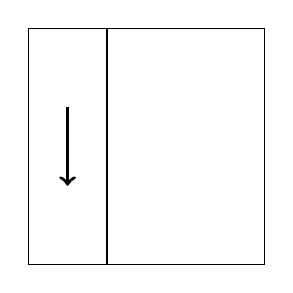
\begin{tikzpicture}[baseline={([yshift=-.5ex]current bounding box.center)}]
        \draw (0, 0) rectangle (1, 3);
        \draw (1, 0) rectangle (3, 3);
        \draw[very thick, ->] (0.5, 2) -- (0.5, 1);
    \end{tikzpicture}
\end{center}

This means that we turn the left face down.

Notice that after four turns, we have returned to the beginning, so 
\[aaaa = a^4 = e\]
which creates a (cyclic) subgroup of the cube,
\[H = \{e, a, a^2, a^3\}\]

\textbf{Notation:} Given $G$ and $a \in G$, 
\[\brak{a} = \{a^k, \; k \in \Z\}\]'

\textbf{Why are the symmetries of the cube not a cyclic group?}

There is no generator of order 24. 

OR cyclic groups are abelian. 
\[a^m a^n = a^{m + n} = a^{n + m} = a^n a^m\]

\section*{Lecture 4: Sept 19}
\subsection*{Review}
\textbf{Recall:} A homomorphism is a map $\phi: G_1 \to G_2$ such that 
\begin{align*}
    \phi(ab) = \phi(a)\phi(b)\\
    \phi(e_1) = e_2\\
    \phi(g^{-1}) = (\phi(g))^{-1} 
\end{align*}

\textbf{To confirm $H$ is a subgroup:} check that it is closed under multiplication and inverses. You do not need to show associativity because that is always true. 

\textbf{Generators:}
Let $G = \{a, a^2, a^3, \dots\}$ If $a^m = a^n \quad m < n$ then 
\begin{align*}
    a^{n - m} = e\\
    a^k = e \qquad (k=n - m)\\
    (a^{k-1}) a = e\\
    a^{k-1} = a^{-1}
\end{align*}

\textbf{Are Abelian Groups always cyclic?}
\emph{Answer:} No. Counterexample:
\[\Z/2 \times \Z/2 = \{(a, b) | \; a, b \in \Z/2\} = \{(0,0), (0, 1), (1, 0), (1,1)\}\]
has no generator. 

\subsection*{(Left) Cosets}
\textbf{Definition:} Given a group $G$ and a subgroup $H \subset G$, a \emph{left coset} is a set of the form 
\[aH = \{ah\; | \; h \in H\}\]
where $a \in G$

If $a \in H$, then $aH = H$. 
(Notice that for all $s \in H$, $a(a^{-1}s) = s$ and $a^{-1}s \in H$)

This all leads to the observation that \emph{every set of cosets contains the subgroup.}

\textbf{Lemma:} $H$ and $aH$ are the same size (there is a bijection from $H$ to $aH$)

\emph{Proof:} Define $\psi(h) = ah$. By definition, $aH = \psi(H)$ so $\psi$ is onto. Now suppose $\psi(h_1) = \psi(h_2)$. Then $ah_1 = ah_2$ which by cancellation shows $h_1 = h_2$. Thus, $\psi$ is one-to-one. Therefore, $\psi: H \to aH$ is a bijection. $\qed$

\textbf{Lemma:} If $aH \cap bH \neq \emptyset$, then $aH = bH$.

\emph{Proof:} Pick an element in common: $ah_1 = bh_2$. Then 
\[a = bh_2h_1^{-1}\]
so for any $h\in H$,
\[ah = b(h_2 h_1^{-1}h) \in bH\]
Since this is true for all $h \in H$, we know that $aH \subset bH$. 

Interchanging $a$ and $b$ shows that $aH = bH. \qed$

\subsection*{Lagrange's Theorem}
\textbf{Theorem:} If $G$ is a finite group and $H \subset G$ is a subgroup, then $o(H) |\; o(G)$ (The order of $H$ divides the order of $H$.) 

\emph{Proof:} Look at all the cosets and denote the number of cosets $n$. We know
\begin{enumerate}
    \item For any $g\in G$, $g=ge \in gH$ (every element is in a coset)
    \item All cosets have $o(H)$ elements (from the bijection)
    \item The cosets are mutually exclusive
\end{enumerate}
So $o(G) = n \cdot o(H) \qed$

\textbf{Corollary:} If $g \in G$ and $G$ is a finite group, then $o(g) | o(G)$

\emph{Proof:} Let $H = \brak{g}$. Then $o(H) = o(g)$. Since $o(H) |\; o(G)$ (by Lagrange's), $o(g) |\; o(G). \qed$

\section*{Lecture 5: Sept 21}
\subsection*{Recall}
\textbf{Lagrange's Theorem:} $H \subset G \implies o(H) |\; o(G)$

\textbf{Corollary of Lagrange's Theorem:} if $g \in G$, $o(g) |\; o(G)$

\subsection*{Equivalence Relations}
\textbf{Relation:} a relation on a set $S$ is a subset $R \in S \times S$
\[x \; R \; y \implies (x, y) \in R\]

\textbf{Equivalence Relation:} a relation $x \sim y$ such that $(x, y) \in R$ and 
\begin{enumerate}
    \item $x \sim x \quad \forall x \in S$
    \item $x \sim y \implies y \sim x \quad \forall x, y \in S$
    \item $x \sim y, \; y \sim z \implies x \sim z \quad \forall x, y, z \in S$
\end{enumerate}

\textbf{Example:} $H \subset G$ with $a \sim  b$ if $a^{-1} b \in H$ 

\begin{align}
    a \sim a &\implies a^{-1}a \in H \implies e \in H \checkmark\\
    a \sim b &\implies a^{-1}b \in H \implies (a^{-1}b)^{-1} = (b^{-1}a)^{-1} \implies b \sim a \checkmark\\
    a\sim b, \; b \sim c &\implies a^{-1}b, b^{-1}c \in H \implies a^{-1}x \in H \implies a \sim c \checkmark
\end{align}

\textbf{Remark:} if two equivalence classes overlap, they are the same 
\emph{Proof:} an equivalence class is a coset 

\textbf{Example:}
\begin{align*}
    a^{-1}b \in H\\
    a^{-1}b = h \in H\\
    b = ab \in aH
\end{align*}

\subsection*{The group $(\Z/n)^*$}
\textbf{Relatively Prime:} $a, b \in \Z$ are \emph{relatively prime} if $\gcd(a, b) = 1$

\textbf{Lemma:} if $a, b$ are relatively prime then $\exists s, t$ such that 
\[as + bt =1\]

\emph{Proof:}

$\impliedby$ suppose $as + bt = 1$ and $d$ divides $a, b$. Clearly, $d | as$ and $d | bt$ for $s, t\in \Z$. By distribution, 
\[d| as + bt = 1 \implies d | 1 \implies d = 1\]

$\implies$ Let $a, b$ be the smallest pair with $a < b$. Consider $a, b - a$. If $a$ and $b-a$ are relatively prime, then 
\[s'a + t'(b- a) = 1 = (\underbrace{s'- t'}_s) a + \underbrace{t'}_tb = 1\]

To show that $a$ and $b- a$ are relatively prime, we suppose $d | a$ and $d | b-a$ so $d | a + (b-a)$ so $d |b$. Using the first part of the proof, we know have $as + bt =1$ for the smallest pair we did not know we could write that way. Thus it is true for all numbers.

\textbf{Definition:} $(\Z/n)^*$ is the subset of $\{1, \dots, N\}$ which is relatively prime to $N$ together with group law multiplication and reduction.
\[(\Z/15)^* = \{1, 2, 4, 7, 8, 11, 13, 13, 14\}\]

\emph{Example:} $7\cdot 8 = 56 - (15*3) = 11 \in (\Z/15)^* $

We now consider $a, b \in (\Z/15)^*$ 
\[\begin{cases}
    1 = s_1 a + t_1 N\\
    1 = s_1 b + t_2 N\\
    1 = s_1 s_av + \dots N
\end{cases} \implies ab \in (\Z/15)^*\] 
(so identity)

\textbf{Inverses in $(\Z/N)^*$:}
\begin{align*}
    a \in (\Z/15)^*\\
    as + tN = 1\\
    s = a^{-1}\\
    aa^{-1} + tN = 1
\end{align*}
(so inverses mod multiples are in the group)

\textbf{Order of $(\Z/15)^*$:} 
\[\phi(n) := o(\Z/15)^*\]

We have $\phi(15) = 8$, $\phi(17) = 16$, etc.

In general, if $p$ is prime then $\phi(p) = p -1$ and if $p, q$ are prime then $\phi(pq) = (p - 1)(q - 1)$

\[\boxed{\frac{\phi(N)}{N} = \prod_{p | n} 1 - \frac{1}{p}}\]
\emph{Example:} $N=12, \quad (\Z/12)^* = \{1, 5, 7, 11\}$
\[\frac{\phi(12)}{12} = (1 - \frac{1}{2})(1 - \frac{1}{3}) = \frac{1}{3} \implies \phi(12) = 4\]

\subsection*{RSA Cryptography}
\textbf{Corollary of Lagrange's Theorem:} If $a$ is relatively prime to $N$ then 
\[a^{\phi(N)} \equiv 1 \mod n\]

\textbf{The Algorithm:}
\begin{enumerate}
    \item Pick two very large primes $p, q$ (choose very big numbers and check if they are prime)
    \item publish the value of $N = pq$ 
    \item Keep secret the number $\phi(N) = (p-1)(q-1)$
    \item Choose a public $E$ relatively prime to $\phi(N)$ ($DE + k\phi(N) = 1$) where $D$ is your private ``decoder''
\end{enumerate}

\chapter*{Rings}
\section*{Lecture 6: Sept 26}
\textbf{Ring:} a set $R$ with two operations (usually $+$, \; $\cdot$) such that:
\begin{enumerate}
    \item $(R, +)$ is an abelian group 
    \item $(R, \cdot)$ is a ``group'' which may or may not have inverses (the operation is always defined, it is associative, and there is an identity) 
    \item 
    \[\forall a, b, c \in R : \quad \begin{cases}
        a \cdot (b + c) = a\cdot b + a \cdot c\\
        (b + c) \cdot a = b\cdot a + c\cdot a
    \end{cases}\]
\end{enumerate}

We usually call $1$ the multiplicative identity (the identity for the operation $\cdot$) and $0$ the additive identity (the identity for $+$)

\textbf{Lemma:} $0 \cdot a = a\cdot 0 = 0 \quad \forall a \in R$

\emph{Proof:} 
\[0 + 0 = 0 \implies (0 + 0)\cdot a = 0a + 0a = 0 \cdot a\]
By the additive inverse,
\[-0a + 0a + 0a = -0a + -0a \implies 0a = 0 \qed\]

\textbf{Lemma:} $(-a) \cdot b = -(a\cdot b)$

\emph{Proof:} 
\begin{align*}
    0 \cdot b &= 0\\
    (-a + a) \cdot b &= 0\\
    -a\cdot b + a\cdot b &= 0\\
    -a \cdot b + a\cdot b -(a\cdot b) &= -(a\cdot b)\\
    -a \cdot b &= -(a \cdot b) \qed
\end{align*}

\subsection*{Examples of Rings}
\begin{itemize}
    \item The integers $(\Z, + , \cdot)$
    \item $\Z/n$
    \item $Z[x]$ (the set of integer polynomials $a_0 + a_x + \dots + a_nx^n$)
    \item $\Z/6[x]$ (polynomials with coefficients in $\Z/6$)
    \item $(R[x])[y]$ (the ring of polynomials in $y$ whose coefficients are elements in $R[x]$)
    \item $R[x, y] = \{\sum a_{ij} x^i y^k | \; a_{ij} \in R\}$ (this is isomorphic to the example above)
    \item $M_n(R)$ is the $n \times n$ matrix ring with coefficients in $R$
    \item $\Z[i] = \{a + bi | \; a, b \in \Z, i^2 = -1\}$ (the Gaussian integers)
    \item $\Z[\omega] = \{a + b\omega\; | \; \omega = e^{2\pi i/3}\}$ (Eisenstein integers)
\end{itemize}

\subsection*{Ring Homomorphisms}
\textbf{Definition:} $\phi: R_1 \to R_2$ is a ring homomorphism iff 
\begin{enumerate}
    \item $\phi(a + b) = \phi(a) + \phi(b)$
    \item $\phi(ab) = \phi(a)\phi(b)$
    \item $\phi(1) = 1$
\end{enumerate}

\textbf{Examples of homomorphisms:}
\begin{itemize}
    \item $\phi: \Z \to \Z/n \longrightarrow \phi(k) = k\mod n$ 
    \item $\phi: \Z/mn \to \Z/n$ 
    \begin{center}
        \begin{tabular*}{0.85in}{|c|c|}
            $\Z/6$ & $\Z/3$\\
            \hline
            $0$ & $0$\\
            $1$ & $1$\\
            $2$ & $2$\\
            $3$ & $0$\\
            $4$ & $1$\\
            $5$ & $2$\\
            \hline
        \end{tabular*}
    \end{center}
\end{itemize}

\section*{Lecture 7: Sept 28}
\subsection*{Review}
\textbf{Ring:} a set with two operations $(R, +, \cdot)$ where $(R, +)$ is an abelian group, $(R, \cdot)$ follows all the group axioms except (potentially) inverses, and 
\[a(b+c) = ab + ac\]

\textbf{Ring Homomorphism:} $\phi: R_1 \to R_2$ where 
\begin{align*}
    \phi(a + b) &= \phi(a) + \phi(b)\\
    \phi(ab) &= \phi(a)\phi(b)\\
    \phi(1) &= 1
\end{align*}

\textbf{More examples:}
\begin{itemize}
    \item $\phi: \Z \to R_2$ is a unique homomorphism ($\phi(1) = 1$, $\phi(2) = \phi(1 + 1) = \phi(1) +\phi(1) = 2, \dots$)
    \item Similarly, (if it exists) $\Z/n \to \R$ will be unique 
    \item $\phi: \mathbb{C} \to \mathbb{C}$. One homomorphism is $\phi(x + iy) = x + iy$. But $\phi(x + iy) = x - iy$ is also a homomorphism
    
    \emph{Lemma:} $\phi(ab) = \phi(a)\phi(b)$

    \emph{Proof:}
    \begin{align*}
        (a+bi)(c+ di) &= ac - bd + i(ad + bc)\\
        (a- bi)(c -di) &= ac - bd - i(ad+bc_)
    \end{align*}

    \item $\Z[\sqrt 2] = \{a + b\sqrt 2 \; | \; a, b\in \; | \;Z\}, \; \phi(a + b\sqrt 2) = a - b\sqrt 2$
\end{itemize}

\subsection*{Unit group}
\textbf{Unit:} an element of a commutative ring with an inverse. i.e.,
\[a, b \in R: ab = 1 \]

\textbf{Lemma:} $(R^\star, \cdot)$ is a group (where $R^\star$ is the set of units of $R$)

\emph{Proof:}
\begin{enumerate}
    \item The units are closed under composition 
    \[1 = aa' = bb' \implies 1 = aa'bb' = (ab)(a'b')\]
    \item $R^\star \subset R$ is a ring so associativity holds
    \item We have an identity because $1 \in R^\star$
    \item We have inverses because $ab = 1 \implies ba=1$
\end{enumerate}

\textbf{Example:} $(\Z/N)^\star = \text{set of elements relatively prime to N}$

Because $(\Z/N)^\star$ is a group, all its elements have inverses so 
\[(\Z / N)^\star \subset (\Z/N)^\sharp\]
(where $(\Z/N)^\sharp$ is the unit group)

Now let 
\begin{align}
    ab = 1 \quad \in \Z/N\\
    b = kN + 1 \quad \in \Z\\
    ab - KN = 1 \implies \text{$ab$ is relatively prime to $N$}
\end{align}
So $a$ is relatively prime to $N$ so
\[(\Z/N)^\sharp \subset (\Z/N)^\star \implies (\Z/N)^\sharp = (\Z/N)^\star\]

\subsection*{Products of Rings}
\textbf{Definition:}
\[R_1 \times R_2 = \{(a_1, a_2) \; | \; a_1 \in R_1, \; a_2\in R_2\}\]
with 
\begin{align}
    (a_1, a_2) + (b_1, b_2) &= (a_1 + b_1, a_2 + b_2)\\
    (a_1, a_2) \cdot (b_1, b_2) &= (a_1 b_1, a_2 b_2)
\end{align}

\textbf{Lemma:} $(R_1 \times R_2^\star) = R_1^\star \times R_2^\star$

If we have units in $R_1, R_2$, then 
\[(a_1, a_2) \cdot (b_1, b_2) = (1, 1)\]

\section*{Lecture 8: Oct 3}
\subsection*{Special Cases of Rings}
\textbf{Field:} $(R - \{0\}, \cdot) = R^*$ is an abelian group (every non-zero element has an inverse)

\textbf{Integral Domain:} A commutative ring where $ab = 0 \implies a = 0 \text{ or } b = 0$

\subsection*{Ideals}
\textbf{Definition:} An \emph{ideal} $I \subset R$ is a subgroup under addition of $R$ and has the ``absorption property'' such that 
\[\forall a \in I, r \in R: ar \in I \]

\emph{Not an Ideal:} 
\begin{itemize}
    \item $I = \R$, $R = \R[x]$
    \item $I = \{(n, n) \big\vert n\in \Z\}, \; R = \Z \times \Z$
\end{itemize}

\emph{Ideals:}
\begin{itemize}
    \item $I = 2\Z, \quad R = \Z$
    \item $I = \{(n, 0) \big\vert n \in \Z\}, \quad R = \Z \times \Z$
\end{itemize}
\vspace{0.25in}

\textbf{Principal Ideals:} Given $a \in R$, 
\[aR = \{ar \; | \; r \in R\}\]

\emph{Proof this is an ideal:}
\begin{itemize}
    \item Distribution: $ab_1 + ab_2 = a(b_1 + b_2)$
    \item Absorption: $s \in R, \; s(ar) = a(sr)$
    \item Inverse: $-ab = a(-b)$
    \item Additive identity: $a0 = 0$
\end{itemize}

\emph{An ideal that is not a principal ideal:}
\begin{itemize}
    \item (General case) All finite sums $\sum_i a_i r_i$ with $a_1, \dots, \; a_n, r_i \in R$ 
    
    Observe 
    \[r\left(\sum_i a_i r_i\right) = \sum_i a_i (rr_i)\]

\end{itemize}

\subsection*{Quotients}
\textbf{Quotient ring:} a ring $\R/I$ from commutative ring $R$ and ideal $I \in R$ 

The elements of $R/I$ are the cosets of $I$,
\[a + I, \quad a \in R\]

We have new group laws:
\begin{align*}
    (a + I) + (b + I) := (a + b) + I\\
    (a + I)(b + I) := (ab) + I
\end{align*}

\emph{Problem:} what if $a$ and $b$ are redundant sets? When $R = \Z$, $I = 2\Z$ we have $1 + 2\Z = 13 + \Z$ (the odd integers) but $1 \neq 13$

\textbf{Lemma:} If $a' +I = a+ I$ and $b' + I = b + I$ then 
\[(a + b) + I = (a' + b') + I\]

\emph{Proof:}
\begin{align*}
    a' = a+ i \qquad i \in I\\
    b' = b +j \qquad j \in I\\
    a' + b' \in (a' + b' + I)\\
    a' + b' = a + b + (i + j) \in (a + b) + I\\
    (a + b + I) \cap (a' + b') + I \neq \emptyset\\
    \therefore (a + b) + I = (a' + b') + I 
\end{align*}

\textbf{Lemma:} If $a' +I = a+ I$ and $b' + I = b + I$ then  
\[a' b' + I = ab + I\]

\emph{Proof:} 
\begin{align*}
    a' &= a + i \\
    b' &= b + i\\
    a'b' &= (a + i)(b+j)\\
    &= ab + ib + aj + ij
\end{align*}
But by absorption, $ib + aj + ij \in ab + I$. so the rest follows from the same proof as above. 

\emph{Showing Associativity:} 
\begin{align*}
    (a + I + b + I) + c + I &= a + I + (b + I + c + I)\\
    ((a + b) + c) + I &= a + (b + c) + I
\end{align*}

\emph{Identity:} $(a + I) + (0 + I) = a + I$

\emph{Inverse:} $(a + I) + (-a + I) = (a - a) + I = 0 + I$ 
\section*{Lecture 9: Oct 5}
\subsection*{Review}
\textbf{Ideal:}

In a commutative ring, $I \subset R$ is an \emph{ideal} if $I$ is a subgroup under addition and $I$ has the absorber property 
\[ar \in I, \quad \forall a\in I, r \in R\]

\vspace*{0.25 in}

\textbf{Quotient:}

We can then construct $R/I$ which is the set of cosets of $I$ (as an abelian group)
\[R/I = \{a + I, \quad a \in R\}\]
However, this construction can obscure the fact that a single coset can be constructed in many ways (for example with $I = 2\Z$, both $0 + I$ and $-30 + I$ are the evens).

Thus we confirm that the operations 
\begin{align*}
    (a + I) + (b + I) := (a + b) +I\\
    (a + I) \cdot (b + I) := ab + I
\end{align*}
on $R/I$ are well-defined (because two cosets that overlap are the same)

\emph{Examples:}
\begin{itemize}
    \item $R/I = \Z/5\Z$ has five distinct cosets:
    \[0 + 5\Z, \; 1  +5\Z, \; 2  +5\Z, \; 3  +5\Z,\; 4 + 5\Z\]
    so it is isomorphic to $\Z/5 = \{0, 1, 2, 3, 4\}$
    
    \item 
    \[R = \R[x] = \left\{\sum_{i=0}^n a_i x^i : \quad a_i \in \R, n \in \{0, 1, 2, \dots\}\right\}\] 
    with 
    \[I = R(x^2 + 1) = \{p(x)(x^2 + 1), \; p(x)\in R\}\] 
    gives the quotient ring $R/I$ with elements like
    \[\begin{cases}
        n + I \quad \forall n \in \mathbb{N}\\ 
        -x^2 + I = -x^2 + (x^2 + 1) + I = 1 + I\\ 
        (x^3 - 5) + I = (x^2 + I)(x + I) + (-5 + I) = (-1 + I)(x + I) + (-5 + I)\\
        \vdots
    \end{cases}\]
    More operations lead to the very strong conclusion: \emph{every ideal can be written in the form}
    \[\boxed{(a + I) + (bx + I) \quad a, b \in \R}\]

    If we continue with this example, we can see 
    \[(x + I)(x + I) = x^2 + I = -1 + I\]
    so in a sense $(x + I) = \sqrt{-1}$ and in fact this does define a ring isomorphism to the complex numbers! 

    \item $R = \mathbb{Q}[x]$ and $I = R(x^2- 2)$ allows us to define ``$\sqrt{2}$''via 
    \[(x + I)(x + I) = x^2 + I = x^2 - (x^2 - 2) + I = 2 + I\]
    This particular ring also happens to be a field.
\end{itemize}
\vspace*{0.25 in}

\textbf{Principal Ideal:} the set of all multiples of an element in the ring 

\subsection*{Homomorphisms and Ideals}
\textbf{Ring homomorphism:} a map $\phi: R_1 \to R_2$ which respects both rings' operations:
\begin{align*}
    \phi(a + b) = \phi(a) + \phi(b)\\ 
    \phi(ab) = \phi(a)\cdot \phi(b)\\ 
    \phi(1) = 1
\end{align*}

\textbf{Kernel:} 
\[\ker(\phi) = \{a \in R_1 \; | \; \phi(a) = 0\}\]

\vspace*{0.25in}
\textbf{Lemma:} $\ker(\phi)$ is an ideal

\emph{Proof:} $\ker(\phi)$ is an abelian group since $\phi$ is also group homomorphism. Let $a \in I, r \in R$. Observe
\begin{align*}
    \phi(ar) &= \phi(a)\phi(r) \quad \text{ring homomorphism}\\ 
    &= 0\cdot \phi(r) \quad a \in \ker\phi\\ 
    &= 0 
\end{align*}
So $ar \in I$. Thus $\ker\phi$ is an abelian group with absorption so it is a group. 

\textbf{Example:}

Given $R$ and $I$ ideal, we construct 
\[\pi: R \to R/I \implies \phi(a) = a + I\] 
Therefore, $\ker \pi = I$

This can also be represented:

\begin{center}
    \begin{tikzpicture}
        \node (R1) at (0,5)  {$R_1$};
        \node (R1/I) at (0, 0) {$R_1/I$};
        \node (R2) at (5, 5) {$R_2$};
        \draw[->] (R1) -- (R2) node[xshift=-1in, yshift=0.2in] {$\phi$};
        \draw[->] (R1) -- (R1/I) node[yshift=1in, xshift=-0.2in] {$\pi$};
        \draw[->, dashed] (R1/I) -- (R2) node[yshift=-1in, xshift=-0.7in] {$\alpha$};
    \end{tikzpicture}
\end{center}

with $I = \ker \phi$.

Does $\alpha$ exist? Observe:
\begin{align*}
    \alpha(a + I) &= \phi(a)\\ 
    \alpha(a' + I) &= \phi(a')\\ 
    a' &= a + i \quad i \in I = \ker \phi\\ 
    \phi(a') &= \phi(a + i) = \phi(a) + \phi(i) = \phi(a) + 0 \phi(a)
\end{align*}
So the map $\alpha$ exists. 

In fact, 
\[\alpha(a + I) = 0 = \phi(a) \implies a \in \ker \phi = I\]
Thus 
\[\ker \phi = \{I\} = 0\]
so $\phi$ iś injective. 

\textbf{Theorem:} If $\phi: R_1 \to R_2$ is onto (surjective) $\alpha: R_1/I \to R_2$ is an $R_2$

\emph{Example:} $R_1 = \R[x]$, $R_2 = \mathbb{C}$, and $\phi: R_1 \to R_2$. 
\[\phi\left(\sum_{k=0}^n a_k x^k\right) = \sum_{k=0}^n a_k i^k = x + iy\]
So 
\[\ker \phi = \{0,\; x^2 + 1, \; p(x)(x^2 + 1)\} = R_1(x^2 + 1)\]
(0 obviously, $x^2 + 1 = i^2 + 1 = 0$, and any multiple of $0$)

Thus, 
\[\R[x]/(\R[x](x^2+1)) \approxeq \mathbb{C}\]

\textbf{Corollary:} In general, $\alpha: R_1/I \to \text{Im}(\phi)$ (where $\text{Im}(\phi) = \phi(R_1)$) is an isomorphism. 

\section*{Lecture 10: Oct 10}
\begin{center}
    \begin{tabular}{|c|c|}
        \hline 
        2 special kinds of Rings & 2 special kinds of Ideals\\ 
        \hline
        Integral domains & Prime ideals\\ 
        Fields & Maximal Ideals\\
        \hline
    \end{tabular}
\end{center}
Unsurprisingly, they are related! We will take them one-by-one and then connect them. 

\textbf{Integral Domain:} $R$ is an integral domain if  
\[\forall a, b \in R: \quad ab = 0 \implies a = 0 \text{ or } b = 0\]

\emph{Not every ring is an integral domain.} Consider $\Z/6$: $2 \cdot 3 = 0$

\textbf{Prime Ideal:} $I \subset R$ is a prime ideal if 
\[\forall a, b \in R: \quad ab \in I \implies a\in I \text{ or } b \in I\]

\emph{Examples:}
\begin{itemize}
    \item $R = \Z, I = 2\Z$ is a prime ideal (product of an even and odd or even and even is even)
    \item $R = \Z, I = 10\Z$ is NOT a prime ideal ($2 \not \in I, 5 \not \in I, 10 \in I$)
    \item $R = \Z[i], I = 5R$ is NOT an ideal (despite 5 being prime) because $1 \pm 2i \not \in I, (1 + 2i)(1-2i) = 5 \in I$
\end{itemize}

Generally, $n\Z$ is a prime ideal precisely when $n$ is prime. 
\vspace*{0.25in}

\textbf{Theorem:} $R/I$ is an integral domain if and only if $I$ is a prime ideal. 

\emph{Proof:} 

We want to show that both directions are true. First consider the lemma that $I$ is prime if $R/I$ is an integral domain. 

Suppose $ab \in I$ (so $ab + I = 0 + I$). We seek to show that $a = 0$ or $b = 0$. Consider the cosets $a + I$ and $b + I$:
\[(a + I)(b + I) = ab + I = I\]
So 
\[(a + I)(b + I) = 0 + I\]
Since $R/I$ is an ID, $a + I = 0 + I$ or $b + I = 0 + I$ in $R/I$. So either $a \in I$ or $b \in I$. Hence, $I$ is prime. 

To see the other direction, first suppose $I$ is prime. Then $a \in I$ or $b \in I$. So 
\[(a + I)(b + I) = 0 \implies ab + I = 0 + I\]
Thus, $ab \in I$. Since $I$ is prime, $a \in I$ or $b \in I$. This is equivalent to 
\[(a + I = 0 + I) \lor (b + I = 0 + I)\] 
So $a = 0$ or $b = 0$ and $R/I$ is an integral domain. $\qed$

\vspace*{0.25in}

\textbf{Field:} $R$ is a field if $R^* = R - \{0\}$ (i.e. all non-zero elements have inverses)

\emph{Lemma:} $R$ is a field if the only ideals in $R$ are $R, \{0\}$

\emph{Proof:} Suppose $R$ is a field and $I \neq \{0\}$ is an ideal. We want to show that $I = R$. Consider, $a \in I, \; a \neq 0$. Because $R$ is a field, $b = a^{-1}$ exists. Further, 
\[1 = ba \in I \quad (\text{by absorption})\]
for any $r \in R$,
\[r = r1 \in I\]
Therefore, $I = R$. 

Going the other direction, suppose $R$ is a ring whose only ideals in $R$ are $R$ and $\{0\}$. We pick any $a \in R, \; a \neq 0$ and consider $I = aR$. Since
\[a1 = a \in I \quad I \neq \{0\}\]
But if $I \neq \{0\}$, then $I = R$ so $1 \in I$. Then for any $r\in R$, $r1 = r \in I$ so $r = a^{-1}$ exists for any $a$. Thus, $R$ is a field.


\textbf{Maximal Ideal:} $I \subset R$ is a maximal ideal if there are no ideals $J$ with $I \subset J \subset R$ (with these being proper subsets) 

\emph{Examples:} 
\begin{itemize}
    \item $6\Z \subset \Z$ is not a maximal ideal because $6\Z \subset 2\Z \subset \Z$
\end{itemize}


\textbf{Theorem:} $R/I$ is a field if and only if $I$ is maximal.

\emph{Proof:} There is a bijection between the set of ideals of $R$ that contain $I$ ($A$) and the set of ideals of $R/I$ ($B$). (See Lecture 11). Then
\[\text{R/I field} \iff \#B = 2 \iff \#A = 2 \iff \text{I maximal}\]

\emph{Alternative Proof Structure:} 

Suppose $I$ is maximal. We pick an ideal $\overline J$ of $R/I$. We want to show that $\overline J = \{[0]\}$ or $\overline J = R/I$. Consider $\pi: R \to R/I$ whose kernel is just $I$. Let $J = \pi^{-1}(\overline J)$. $J$ is an ideal because it has the absorber property. Further, $I \subset J$ because $I = \ker(\pi)$. Therefore, $I \subset J \subset R$. Since $I$ is maximal, $J = I$ or $J = R$. If $J = I$, then $\overline J = \{[0]\}$. Similarly, if $J = R$, then $\overline J = \pi(R)$. So the only ideals in $R/I$ are $\{0\}$ and $R$. 

To see the other direction, assume the only ideals in $R/I$ are $\{0\}$ and $R$. Try to find a subset $I \subset J \subset R$ with $J \neq I$ and $J \neq R$ but as the \color{red} ... \color{black}

\textbf{Corollary:} $\Z/p\Z$ is a field for $p$ prime. 

\emph{Proof:} Show $p\Z$ is a maximal ideal. 
\[p\Z \subsetneq J \subset \Z\] 
Since $J \neq p\Z$ there must be an element $n \in J$ relatively prime to $p$. Then, 
\[1 = ap + bn\] 
$ap \in J$ because $ap \in p\Z \subset J$ and $bn \in J$ by absorber. Thus $1 \in J$ so $J = (1) = \Z$. 

\section*{Lecture 11: Oct 17}
\textbf{Setup:} $R$ is a commutative ring and $I$ is an ideal of $R$. We have a quotient ring $R/I = \{a + I \; | \; a \in R\}$ and a map $\pi: R \to R/I$ defined by $\pi(a) = a + I = \{a + b \; | \; b - I\}$ 

\begin{center}
    \begin{tikzpicture}
        \draw[blue] (0, 0) circle (3cm) node[xshift=-2cm, yshift=3cm]{$R$};
        \draw[blue, dashed] (0, 0) circle (2cm) node[yshift=2.3cm]{$\pi^{-1}(J)$};
        \draw[blue] (0, 0) circle (1cm) node{$I$};

        \draw[->] (3.2, 0) -- (6.8, 0);

        \draw[red] (10, 0) circle (3cm) node[xshift=-10cm, yshift=10cm]{$R$};
        \draw[red, dashed] (10, 0) circle (2cm) node[yshift=2.3cm]{$J$};
        \draw[red] (10, 0) circle (0.1cm) node[xshift=0.5cm]{$\{0\}$};
    \end{tikzpicture}
\end{center}

\emph{Meadow:} a ring whose only ideals are $(0)$ and $R$; synonymous with field

\textbf{Lemma:} there is an isomorphism between 
\[\overset{A}{\left\{\text{Ideals of $R$ which contain $I$}\right\}} \iff \overset{B}{\left\{\text{Ideals of $R/I$}\right\}}\]

\emph{Proof:} To show there is an isomorphism between $A$ and $B$ it suffices to show that there are maps $f: A \to B$ and $g: B \to A$ where $f^{-1} = g$. 

Take an element $K \in A$. Then $\pi(K)$ is a member of $B$ and we just need to check that $\pi(K)$ is an ideal of $R/I$. Conversely, if $J \in B$, we need to check $\pi^{-1}(J)$ is an ideal of $R$. 

Finally, we just need to check that the functions $\pi$ and $\pi^{-1}$ are in fact inverses:
\[\begin{cases}
    \pi(\pi^{-1}(J)) = J\\
    \pi^{-1}(\pi(K)) = K
\end{cases}\]

\begin{enumerate}
    \item Show $\pi(K)$ is an ideal:
        \begin{align*}
            \pi(0) = 0 \implies &0 \in \pi(K) & \\
            \pi(a) + \pi(b) = &\pi(a + b) \in \pi(K)& \qquad (\pi(a), \pi(b) \in \pi(K) \forall a, b \in K)\\
            -\pi(a) = &\pi(-a) \in \pi(K) &\qquad (\pi \text{ is homomorphism and }  -a \in K)\\
            r\pi(a) = \pi(c)\pi(a) = &\pi(ca) \in \pi(K) &\qquad (r \in R/I \implies r = \pi(c) \; | \; c \in R)
        \end{align*}
    \item Show $\pi^{-1}(J)$ is an ideal: (Basically same proof)
    
    \item Show $\pi(\pi^{-1}(J)) = J$:
        
        By definition of $\pi^{-1}$, $\pi(\pi^{-1}(J)) \subset J$. Then we want show that $J \subset \pi(\pi^{-1}(J))$. Pick $a \in J$. Since $\pi$ is onto, $a = \pi(r), \; r \in R$. Because $\pi(r) \in J$, $r \in \pi^{-1}(J)$. So $a = \pi(r) \in \pi(\pi^{-1}(J))$

    \item Show $\pi^{-1}(\pi(K)) = K$: 
    
        First we show $K \subset \pi^{-1}(\pi(K))$. Pick $a \in K$. Then $\pi(a) \in \pi(K) \implies a \in \pi^{-1}(\pi(k))$ because $a$ has the property that it is mapped into $\pi(K)$ by $\pi$.

        To show $\pi^{-1}(\pi(K)) \subset K$, choose $a \in \pi^{-1}(\pi(K))$. We know $\pi(a) \in \pi(K)$ so $\pi(a) = \pi(b) \; | \; b \in K$ so $\pi(a) - \pi(b) = \pi(a - b) = 0 \implies a - b \in I \implies a -b \in K$ (because $I \subset K$). So $a = (a - b) + b \in K$. 
\end{enumerate}

\chapter*{Fields}
\section*{Lecture 12: Oct 19}
\subsection*{Review}
There is a bijective map between the set of ideals of $R$ that contain $I$ and the ideals of $R/I$ given a homomorphism $\pi: R \to R/I$

\textbf{Theorems:}
\begin{itemize}
    \item $R/I$ is an integral domain if and only if $I$ is a prime ideal
    \item $R/I$ is a field if and only if $I$ is maximal 
\end{itemize}

\subsection*{Defining Fields} 
A field is:
\begin{itemize}
    \item A ring where every non-zero element has an inverse 
    \item A ring whose only ideals are $R$ and $\{0\}$
    \item The quotient $R/I$ if and only if $I$ is maximal
    \item A ring with division and commutativity
\end{itemize}

\subsection*{Example of Fields:}
\begin{itemize}
    \item $\mathbb{Q}$ - the rational numbers 
    \item $\R$ - the real numbers 
    \item $\mathbb{C}$ - complex numbers ($x + yi \; | \; x, y \in \R$ i.e., the set of linear combinations of $x$ and $i$)
    \item $\mathbb{Q}[\sqrt 2] = \{a + b\sqrt 2 \; | \; a,b\in \mathbb{Q}\}$ (\emph{Proof:} $(a + b\sqrt 2)(a - b\sqrt 2) = a - 2b^2$)
    \item $\mathbb{Q}[\sqrt D]$ (if $D$ is not a perfect square)
    \item $\Z/p\Z$ if $P$ is prime (because $p\Z$ is maximal)
    \item $F =\{a + b \diamond \; | \; a, b \in \Z/3\} = \Z/3[x]/(x^2 -2)\Z/3[x]$ where $\diamond^2 = 2$ in $\Z/3$ (this set has $9$ elements because $a$ and $b$ each have three values)
\end{itemize}

\textbf{Interlude:} Constructing the rational numbers 

\[\mathbb{Q} = a \star b , b \neq 0, a_1 \star b_1 \sim a_2 \star b_2 \iff a_1b_2 = a_2b_1\]
with multiplication defined on the equivalence class of quotients 
\[[a_1 \star b_1] [a_2 \star b_2] = [a_1a_2 \star b_1 b_2]\]
and addition defined  
\[[a_1 \star b_1] + [a_2 \star b_2] = [a_1b_2 + a_2b_1 \star b_1 b_2]\]

Note that $\star$ is an operation that functions exactly like division but is meant to emphasize that it carries no other intrinsic properties except these operations on equivalence classes. 

\subsection*{Vector spaces}
\textbf{Definition:} a set $V$ is a \emph{vector space} over a field $\mathbb{F}$ if 
\begin{enumerate}
    \item $V$ is an abelian group (under addition)
    \item $(a+ b) \vec v = a\vec v + b\vec v \quad \forall a,b \in \mathbb{F}, \vec v \in V$
    \item $(ab) \vec v = a(b\vec v) \quad \forall a, b \in \mathbb{F}, \vec v\in V$
    \item $a(\vec w + \vec w) = a\vec v + a \vec w \quad \forall a \in \mathbb{F}, \vec v, \vec w \in V$
\end{enumerate}

\textbf{Examples:} 
\begin{itemize}
    \item $\R^n$
    \item $\mathbb{C}^n$
    \item $\mathbb{Q}^n$
    \item (Extension Field) Given fields $\mathbb{F} \subset K$, $K$ (the extension field) is a vector space over $\mathbb{F}$ (the subfield)
    \item $\mathbb{C}$ is a vector space over $\R$ 
    \item $\R$ is a vector space over $\mathbb{Q}$
    \item $\Q[\sqrt 2]$  is a vector space over $\Q$
    \item $\Z/\Z[\diamond]$ is a vector space over $\Z/3\Z$
\end{itemize}

\textbf{Linear combinations of $v_1, v_2, \dots, \; v_n \in V$}:
\[sum_{i=1}^n a_i v_i \quad a_i \in \mathbb{F}\]

\textbf{Spanning set:} $\{v_i\}$ is a spanning set if every $v \in V$ is a linear combo of $\{v_i\}$

\textbf{Independent set:} $\{v_i\}$ is an independent set if 
\[\sum_{i=1}^n a_i v_i = 0 \implies a_1, \dots, \; a_n = 0\]

\textbf{Basis:} $\{v_i\}$ is a basis if it is an independent spanning set

\textbf{Theorem:} If $V$ has a finite basis, then all bases have the same number of elements (which we call $\dim(V)$)

\textbf{Axiom of Choice:} postulate that every vector space has a basis 


\section*{Lecture 13: Oct 24} 
    \textbf{Notation:} $F[x]$ is ring set of polynomials with coefficients in $F$

    \subsection*{Long division of polynomials}
    \textbf{Theorem: (Division Algorithm)} 

        Suppose you have two polynomials 
        \begin{gather*}
            p(x) = a_m x^m + \dots + a_1, \quad a_i \in F, a_m \neq 0\\
            q(x) = b_n x^n + \dots + b_1, \quad b_i \in F, b_n \neq 0
        \end{gather*}
        (We say $\deg(p) = m$ and $\deg(q) = n$)

        Then $q(x) = a(x)p(x) + r(x)$ where $\deg(r) < \deg(p)$

    \emph{Proof:} Induction on $n - m$

        Base case: $n - m < 0$ so $q = 0p + r$ 

        Generally,
        \[q_* = q - \frac{b_n}{a_m} x^{n - m} p(x) \qquad \deg(q_*) = n_* < n\]

        By induction,
        \[q_* = a_* p + r \qquad \deg(r) < \deg(p)\]
        so 
        \[q - \frac{b_n}{a_m} x^{n - m} p(x) = a_* p + r \implies q = (\underbrace{a_* + \frac{b_n}{a_m} x^{n - m}}_a)p + r \qed\]

    \subsection*{Theorems of Polynomial Rings}
    \textbf{Theorem:} All ideals in $F[x]$ are principal

        \emph{Proof:} Let $I$ be an ideal. Consider $p(x) \in I$, the smallest degree non-zero polynomial in $I$. Let $q \neq 0 \in I$. By the division algorithm,
            \[q = ap + r \quad \deg r < \deg p\]
        Since $r = q - ap$, and $I$ is ideal, $r \in I$. Therefore, $\deg r = 0$ (or else it would be smaller than $p$). Thus, $q = ap$ which is a contradiction. 

    \textbf{Definition:} $p(x) \in F[x]$ is \emph{irreducible} if $p(x) = a(x)b(x) \implies \deg(a) = 0 \lor \deg(b) = 0$

    \textbf{Theorem:} if $p(x) \in F[x]$ is irreducible, then $I = p(x)F[x]$ is maximal

        \emph{Proof:} Let $J = b(x)F[x]$ be an ideal such that $I \subseteq J \subseteq F[x]$. We know $p \in J$ because $p \in I$. So 
        \[p(x) = a(x)b(x)\]

        Case 1: $\deg(a) = 0$ so $p = b$ up to constants and $I = J$

        Case 2: $\deg(b) = 0$ so $1 \in J \implies J = F[x]$ (because inverse of $b \in F[x]$)

    \textbf{Theorem:} $F[x]/p(x)F[x]$ is a field. 

        \emph{Proof:} Given $c \in F$, consider the coset $[c] = c + p(x)q(x)$. We define a ring homomorphism $\phi: F \to F/p(x)F[x], c \mapsto [c]$. 
        
        Suppose $c \in \ker\phi$. Then 
        \[[c] = [0] \implies c \in p(x)F[x] \implies c = a(x)p(x) \implies a(x) = c \implies c = 0\]
        So $\ker \phi = 0$. Then by the isomorphism theorem, $F$ is isomorphic to $\phi(F)$ which means that $\phi(F)$ is a field.

    \textbf{Theorem:} $F[x]/p(x)F[x]$ contains a root of $p(x)$

        \emph{Proof:} Consider $[x] = x + p(x) F[x]$. Since $\phi(F)$ contains a copy of $F$ (mapped to its cosets), we can write 
        \[p([x]) = [p(x)] = [0]\]
        by using the formula for coset composition. 

\section*{Lecture 14: Oct 26}
    \subsection*{Review}
        \textbf{Polynomial division:} we can write any polynomial $q = ap + r$ where $\deg r < \deg p$

        \textbf{Theorems:}
        \begin{itemize}
            \item if $F$ is a field, all ideals in $F[x]$ are principal 
            \item If $p \in F[x]$ is irreducible, then $I = p(x)F[x]$ is maximal 
            \item $F[x]/p(x)F[x]$ is a field (look at the map $\phi: F \to F[x]/p(x)F[x],\quad a\mapsto [a] = a + p(x)F[x]$)
            \item $F[x]/p(x)F[x]$ contains a root of $p(x)$
            
            \indent \emph{Proof:}
            \begin{gather*}
                p(x) = a_0 + \dots + a_nx^n \in F[x]\\
                p(x) = [a_0] + \dots + [a_n] x^2 \in K[x]\\
                p([x]) = [a_0] + \dots + [a_n][x]^2 = [a_0 + a_1x + \dots a_nx^b] = [p(x)] = [0] \in K
            \end{gather*}
        \end{itemize}

        \textbf{An Example:} $F= \R, \quad p(x) = x^2 + 1, \quad K = R[x]/(x^2 + 1)R[x]$
            We know $x^2 + 1$ is irreducible because $\sqrt{-1} \not \in \R$. We then consider the map $r \to [r]$ so 
            \begin{gather}
                [x]^2 + [1] = 0\\
                [x]^2 = [-1]
            \end{gather}
            We define $i := [x]$ so $i^2 = -1$. Further, 
            \[[x] + i[y] \in K\]
            for amy element in $k$ because 
            \[[x^n] = [x^2][x^{n-2}] = [-x^{n-2}]\]
            so we can factor down any polynomial to lowest degree.

    \subsection*{Bases}
        \textbf{Basis:} a linearly independent spanning set
        
        \textbf{Example:} $\{1, i\}$ is a basis of $\C$ over $\R$ 

        \textbf{Example:} Is $S = \{[1], [x], \dots,\; [x^{n-1}]\}$ a basis? 
        \indent \emph{Proof:} It is a spanning set because 
        \[[x^n] = -\frac{[a_{n-1}] [x^{n-1}]}{[a_n]} \cdot -\frac{[a_0]}{[a_n]}\]

        Suppose it is not linearly independent. then $\exists[b_0], \dots,\; [b_{n-1}]$ such that 
        \[[b_0][x] + \dots + [b_{n-1}][x^{n-1}] = [0]\]
        Using the formula, 
        \[[b_0 + \dots + b_{n-1} x^{n-1}] = [0] = [p(x)]\]
        Since the polynomial is in the ideal, it is a multiple of $p(x)$. But $p$ has degree $n$ and $\deg([b_0 + \dots + b_{n-1} x^{n-1}]) = n -1$. But since $n - 1 < n$, it cannot be a multiple of $p$ so contradiction. 

    \subsection*{Dimensionality}
        Let $\subset K$. Then we denote 
        \[[K : F] = \dim_F K = \text{the dimension of K as a vector space over F}\]

        \textbf{Example:} $[\C : \R] = 2$ (because the basis is $\{1, i\}$)

        \textbf{Example:} $[F[x]/ p(x)F[x] : F] = \deg(p)$

        \textbf{A Homework Problem:} $F = \Q, \; p(x) = x^3 -2$ 
            \[[F[x]/F[x](x^3-2) : \Q] = 3\] 
            (Here $[x] = \sqrt[3]{2}$) and the basis is 
            \[\{[1], [x], [x^2]\} = \{1, \sqrt[3]{2}, \sqrt[3]{4}\}\]

        \textbf{Theorem:} $F \subset K \subset L$, 
        \[[L : F] = [L : K][K : F]\]
            
            \emph{Proof:} Let $m = [K : F], \quad n = [L : K]$. Let $v_1, \dots,\; v_m$ be an $F$-basis for $K$. Let $w_1, \dots,\; w_n$ be a $K$-basis for $L$. We consider the set $\{v_i w_j\}$ and seek to prove that it is a spanning set and linearly independent. 

            \indent \emph{Lemma:} $\{v_iw_j\}$ is a spanning set. 

            \indent \emph{Proof:} Pick an element $l \in L$. It can be written in the form 
            \[l = \sum_i \sum_j k_{ij} v_i w_j\]

            \indent \emph{Lemma:} $\{v_iw_j\}$ is independent 

            \indent \emph{Proof:} Suppose $\sum_{i, j} f_{ij} v_i w_j = 0$. 
            \[\left(\sum_{i} f_{i1} v_i\right)w_1 + \dots +\left(\sum_{i} f_{in} v_i\right)w_n = 0\]
            \indent But the $v_i$ are a basis for $K$ so 
            \[\sum_{i,j} f_{ij} v_i = 0 \implies f_{ij} = 0 \qed\]


\chapter*{Groups - Part II}
\section*{Lecture 15: Oct 31}
    \subsection*{Normal Subgroups}
        Let $G$ be a group and $H \subset G$ be a subgroup. Further, we have two cosets:
        \begin{gather*}
            aH = \{ah \; | \; h \in H\}\\
            Ha = \{ha \; | \; h \in H\}
        \end{gather*}

        \begin{enumerate}
            \item When is $aH = Ha$? 
            \item Is $aH \cdot bH = abH$ well defined?
        \end{enumerate}

        \textbf{Definition:} $H$ is \emph{normal} if $aH = Ha \quad \forall a \in G$

        \emph{Equivalent Definitions:} 
        \begin{itemize}
            \item $H = aHa^{-1} \quad \forall a \in G$
            \item $a^{-1} H a = H \quad \forall a \in G$
            \item $a^{-1}Ha \subset H \quad \forall a \in G$ (\emph{Proof:} $a^{-1}(aha^{-1})a$)
        \end{itemize}

        \textbf{Definition:} we call $aH a^{-1} = H$ the \emph{conjugation} of $H$

        \textbf{Examples of Normal Subgroups:}
        \begin{itemize}
            \item All subgroups of an abelian group are normal 
            \item $\{e\}$ is normal in every group ($e^{-1}He \subset H$)
            \item Any group is a normal subgroup of itself
            \item $\Z/3$ (rotation group) is a normal subgroup of $D_3$
        \end{itemize}

        \textbf{Examples of Non-normal subgroup:}
        \begin{itemize}
            \item The subgroup generated by a flip in $D_3$ is not normal (flips don't commute with rotations)
        \end{itemize}

        \textbf{Lemma:} If $\phi: G_1 \to G_2$ is a homomorphism, then $\ker \phi$ is normal in $G_1$

        \emph{Proof:} It suffices to show that if $h \in \ker(\phi)$ then $ah^{-1}a \in \ker(\phi)$. Observe:
        \[\phi(aha^{-1}) = \phi(a)\phi(h)\phi(a^{-1}) = \phi(a) e_2 \phi(a^-1) = \phi(aa^{-1}) = \phi(e_1) = e_2\]

        \emph{Example:} We always have a homomorphism $\phi: D_n \to \Z/2$,
            \[\phi(g) = \begin{cases}
                0 \quad \text{g is rotation}\\
                1 \quad \text{g is flip}
            \end{cases}\]
        So $\ker \phi = \Z/n$, the rotations. 

    \subsection*{Quotient Construction for Groups}
        We want 
        \[aH \cdot bH = ab \cdot H \quad \forall a,b \in G\] 

        First, we need to check that it is well-defined. Suppose $a'H = aH$. If it is well-defined, then 
        \[a'bH = ab H\]

        Suppose $a' = ah$. Then, $a'bH = ahb H$. Is $ahbh_1 \in abH \quad a,b \in G, h_1 \in H$? 

        Well, clearly, this equivalent to the condition $ahbh_1 = abh_2 \quad h_2 \in H$. Further, 
        \begin{align*}
            hbh_1 &= bh_2 \qquad \text{cancellation}\\
            b^{-1} hbh_1 &= h_2\\
            b^{-1}hb &= h_2h^{-1}\\
            b^{-1}hb &\in H
        \end{align*}

        So, the formula is well-defined when $b^{-1}hb \in H\quad \forall b\in G$. This is precisely when $H$ is normal!

        For the other side, we want to show that $ab'H = abH$ with $b'=bh$:
        \begin{align*}
            abhH &= abH\\
            abhh_1 &= abh_2
        \end{align*}
        But $h_1$ and $h_2$ are arbitrary so $hh_1 = h_2$ by closure. 

        Thus, the formula is well-defined:
        \[aN \cdot bN = ab \cdot N \quad a, b \in G\]
        where $N \subseteq G$ is normal
        and we call the group of cosets of $N$, $G/N$

        Consider, $\pi: G \to G/N$, $\pi(a) = aN$ so $\ker \pi = N$

    \subsection*{Isomorphisms of Normal Subgroups}
        Say we a homomorphism $\phi: G_1 \to G_2$ whose $\ker \phi = N$ 

        \begin{center}
            \begin{tikzpicture}
                \node (G1) at (0,5)  {$G_1$};
                \node (G1/N) at (0, 0) {$G_1/N$};
                \node (G2) at (5, 5) {$G_2$};
                \draw[->] (G1) -- (G2) node[xshift=-1in, yshift=0.2in] {$\phi$};
                \draw[->] (G1) -- (G1/N) node[yshift=1in, xshift=-0.2in] {$\pi$};
                \draw[->] (G1/N) -- (G2) node[yshift=-1in, xshift=-0.7in] {$\alpha$};
            \end{tikzpicture}
        \end{center}

        \[\alpha(a' N) = \phi(a') = \phi(a)\phi(n) = \phi(a) = \alpha(aN)\]

        Further, 
        \[\ker \alpha = \{N\}\]
        (the trivial subgroup of $G/N$)
        because 
        \[\alpha(aN) = e \implies \phi(a) = e \implies a\in \ker \phi \implies a \in N \implies aN = N\]

        so 
        \[\alpha: G/\ker(\phi) \to G_2 \text{ is injective (one-to-one)}\]

        \textbf{Theorem:} 
        \[\alpha: G_1/\ker(\phi) \implies \text{Im}(\alpha) = \text{Im}(\phi) \text{ is an isomorphism}\]

\section*{Lecture 16: Nov 2}
    \subsection*{Review}
        Normal subgroups are those that satisfy 
        \[aN = Na \iff aNa^{-1} = N \iff aNa^{-1} \subset N \quad \forall a \in G\]

        We call the group of cosets of $N$ $G/N$ whose composition is governed by 
        \[aN \cdot bN = ab \cdot N\]


    \subsection*{Cayley's Theorem (12.2)}
        \textbf{Theorem:} Every group is isomorphic to a subgroup of a permutation group 

        \emph{Note on notation:} we could equivalently consider the group of permutations of $S$ (the set of bijections from $S \to S$), the automorphisms on $S$, the maps on $S$, and the bijections on $S$. 

        \emph{Proof:} It suffices to construct a homomorphism from $G \to \text{Per}(G)$ (the permutations of $G$), then show it is injective and apply the isomorphism theorem.

        First given a $g$, define $L_g: G \to G$ rby the formula $L_g(a) = ga$. Now it just remains to show:
        \begin{enumerate}
            \item $L_g$ is a bijection 
            \item $\phi: g \to L_g$ is a homomorphism
            \item $\phi: g \to L_g$ is injective 
        \end{enumerate}

        \indent \emph{Lemma 1:} $L_g$ is a bijection 

        \indent \emph{Proof:} Suppose $L_g(a) = L_g(b)$. Then $ga = gb \implies a = b$ so injective. Further, $\forall a \in G, \quad Lg(g^{-1}a) = g^{-1}ga = a$ so surjective. Thus $L_g$ is a bijection. $\square$

        \indent \emph{Lemma 2:} $\phi(gh) = \phi(g) \phi(h)$, i.e. $L_{gh} = L_g \cdot L_h$

        \indent \emph{Proof:} Let $a \in G$. $L_{gh}a = gha$. 
        \[L_g\cdot L_h(a) = L_g(L_h(a)) = L_g(ha) = gha \quad \square\] 

        \indent \emph{Lemma 3:} $\phi$ is injective. 

        \indent \emph{Proof:} Suppose $L_g = L_h$. Then take 
        \[g = L_g(e) = L_h(e) = h \implies g = h \quad \square\]

        Now by the isomorphism theorem, the map from $g \to L_g$ is an isomorphism. $\blacksquare$

    \subsection*{Cayley Graphs}
        Let $S = a_1, \dots,\; a_n \in G$ be the generating set of $G$. 

        We can create a graph whose vertices are all the elements in the group and where the directed elements go from $g \to ga_i$ for each $a_i \in S$ and $g \in G$. 

        Notice that if we apply a permutation (say $L_g(g) = hg$) then all the edge relations are respected ($hg \to hga_i$). 

        \textbf{Conclusion:} we can extend Cayley's theorem to the group of symmetries of the graph. 

        \textbf{Examples:}
        \begin{itemize}
            \item $G = \Z, \quad S = \{1\}$ generates the whole group 
            \item $G =\Z^2, \quad S = \{(1, 0), (0, 1)\}$ creates the 1x1 grid 
        \end{itemize}

    \subsection*{Group Actions (6.2)}
        \textbf{Definition:} a group action of group $G$ on a set $S$ is a homomorphism from $G$ to $\text{PER}(S)$. 

        Alternatively, a group action of $G$ on $S$ is a map $G \times S \to S$ such that 
        \begin{enumerate}
            \item the map $(g, s) \to g\cdot s$ is a bijection if $g$ is fixed
            \item $gh\cdot s = g\cdot hs \quad \forall g,h \in G \text{ and } s\in S$ (Homomorphism condition)

        \end{enumerate}

        \textbf{Note:} in general, there is no reason to expect their should be a well-defined composition between the elements of the group and the elements of the set. When there is, we have a group action.

        \textbf{Example:}
        \begin{itemize}
            \item $G$ is the invertible linear transformations in $\R^2$ and $S$ is the lines in $\R^2$. If we apply a linear transformation to a line, then we get a new line. 
            \item The set of triangles and the group of linear transformations
            \item The group of symmetries of vertices of a dodecahedron and the set of 5 tetrahedrons created by the vertices
            \item $H \subset G, S = \{aH \; | \; a \in G\}$ so $g\cdot (aH) = gaH$
        \end{itemize}

        \textbf{Definition:} the \emph{orbit} $Gs$ of $s\in S$ is the set $\{g\cdot s \; | \; g \in G\}$

        \textbf{Definition:} the \emph{stabilizer} $\emph{Stab}(s) \subset G$ of $s\in S$ is the set of all $g \in G$ such that $g\cdot s = s$. Note that it is also a subgroup.

\section*{Lecture 17: Nov 5}
    \subsection*{Review}
        \textbf{Group action:} a homomorphism $\phi: G \to \text{PER}(S)$ such that 
        \begin{align*}
            gs &= \phi(g)(s)\\
            ghs &= g(hs)\\
            es &= s \quad \forall s
        \end{align*}

        \textbf{Orbit:} $Ga := \{ga : g\in G\}$

        \textbf{stabilizer:} $S_a = \{g\in G:\; ga = a\} \quad (a\in S)$ 

        \textbf{Lemma:} two orbits are identical or completely disjoint

        \emph{Proof:} Suppose $Ga \cap Gb \neq \emptyset$. Then $ga = hb$ for some $g, h \in G$.
        \begin{align*}
            g^{-1}ga &= g^{-1}hb\\
            a &= g^{-1}hb\\
            a = kb &\implies Ga \subset Gb
        \end{align*}
        Arguing from the other side shows $Ga = Gb. \qed$

        \textbf{Lemma:} the size of the orbit $\#Ga = \frac{\#G}{\#S_a}$

        \emph{Proof:} notice that the quotient is just the number of cosets of $S_a$. So consider any left coset $bS_a$ and we try to map it into $Ga$:
        \[b\cdot S_a \mapsto b\cdot a\]
        We know this is well-defined because if we assume there is some other element of the coset
        \[b'S_a = bg\cdot S_a \quad g\in S_a \implies b'a = bga = ba \]

        Now we define $\psi: \text{cosets of } S_a \to Ga$. Clearly, $\psi$ is onto. Further, it is 1-1: Suppose $\psi(g\cdot S_a) = \psi(h \cdot S_a)$. Thus,
        \[ga = ha \implies a = g^{-1}ha \implies g^{-1}h \in S_a \implies h \in g\cdot S_a\]
        So we conclude that $g\cdot S_a = h\cdot S_a$. We have established a bijection so they have the same number of elements. $\qed$ 

    \subsection*{Sylow's Theorem}
        \textbf{Lemma (Abelian Cauchy):} If $G$ is an abelian group and $p$ is prime and $p \; | \; G$, then $G$ has an element of order $p$. 

        \emph{Proof:} 
        \begin{itemize}
            \item Case 1: $G$ is cyclic ($G = \langle g \rangle, \; g^{o(G)} = e$). Then we can take $h = g^{o(g)/p}$ and $o(h) = p$. 
            \item Case 2: $G$ is not cyclic, so $G$ has a non-trivial subgroup $N$. 
            \begin{enumerate}
                \item $p \; | \; \#N$ so by induction, $\exists g\in N$ s.t. $o(g) = p$
                \item $p \not \mid o(N)$. We are in an abelian group so everything is normal and we can take the quotient: $\overline G = G/N$. By induction, $\exists \overline g\in \overline G$ with order $p$. 
                
                The elements of $\overline G$ look like $gN, g^2N, \dots g^pN$ but $g \not \in N$ and we want $g^p \in N$. If $g^p = e$ we would have an element of order $p$ and we would be done. However, we also need to check the case 
                \[g^p = a \in N\]
                Let $d = o(a)$ so $d$ is relatively prime to $p$ and check 
                \[(g^p)^d = e \implies (g^d)^p = e\]
                So if $g^d \neq e$ we are done. 

                Proof by contradiction: suppose $g^d = e \in N$. Further, $g^p \in N$. 
                By Bezout's,
                \[ap + bd = 1 \implies g = g^1 = g^{ap+bd} = g^{ap}g^{bd}= (g^p)^a(g^d)^b \in N\] 
                so $g^d \neq e$. $\qed$
            \end{enumerate}
        \end{itemize}

        \textbf{Sylow's First Theorem:} Suppose $\#G = p^nk$ and $p$ does not divide $k$. Then $G$ has a subgroup of order $p^n$. 

        \emph{Proof:} Let $G$ be a group of smallest order where we do not know Sylow's theorem is true. 

        Now let $S = G$ be a group action such that $ga = gag^{-1}$. We know this is a group action because:
        \[gha = gha(gh)^{-1} = ghah^{-1}g^{-1} = gha\]

        Now look at all stabilizers $S_a = \{g\in G: gag^{-1} = a\}$. These are going to be subgroups of $G$. 

        Cases:
        \begin{enumerate}
            \item $\#S_a = p^nl, \quad l < k \implies \exists H< S_a$ where $\#H = p^n$ and we are done. 
            \item $\#S_a = p^m l, \quad m < n$
            \item $S_a = G$
        \end{enumerate}

        If $S_a = G$ then $\#G/\#S_a = 1$ so every orbit has one element. These elements form the center of the group because $gag^{-1} = a$ for all $g$. Further, $P$ divides $\#Z$ because for all the cases $\#S_a = p^m l \quad (m < n)$, clearly the order is divisible by $p$. 

        Since the center is abelian, $\exists N \subset Z(G)$ with $\#N = p$ (this subgroup is normal because abelian so $Na= aN$).  

        Now we create the quotient $\overline G = G/N$ and $\#\overline G = p^{n-1}k$. By induction, $\exists \overline H \subset \overline G$ with $\#\overline H = p^{n-1}$ 

        Let $\pi: G \to \overline G$ (this is a p-to-1 map) and let $H = \pi^{-1}(\overline H) \subset G$. Hence, $\# \overline H = p^n. \qed$

\section*{Lecture 18: Nov 9}
    \subsection*{Sylow's Theorems}
        \textbf{Definition:} Let $G$ be a group with order $p^nk$ such that $p \not \mid k$. $H$ is a Sylow p-subgroup if $\#G = p^n$

        \textbf{Sylow's First Theorem:} the number of Sylow p-subgroups is greater than or equal to $1$ (there is always at least one Sylow p-subgroup in $G$)

        \textbf{Sylow's Second Theorem:} any two Sylow p-subgroups are conjugate: for some $g$, 
        \[K = gHg^{-1}\]

        \textbf{Sylow's Third Theorem:} the number of Sylow p-subgroups divides $k$ and is congruent to $1$ mod $p$. 

    \subsection*{Sylow's Second Theorem}
        \textbf{Notation:} 
        \begin{gather*}
            AB = \{ab \; | \; a\in A, b \in B\}\\
            AB = \{abc \; | \; a \in A, b \in B, c \in C\}\\
            AgBhCk = \{agbhck \; | \; a\in A, b \in B, c \in C\}
        \end{gather*}

        \textbf{Lemma:} If $H$ is a subgroup of $G$, $gHg^{-1}$ is a subgroup with $g \in G$.
            \begin{align*}
                gHg^{-1} = \{ghg^{-1} \; | \; h \in H\}\\
                (gh_1g^{-1})(gh_2g^{-1}) = gh_1h_2g^{-1}\\
                (ghg^{-1})^{-1} = gh^{-1}g^{-1} \qed
            \end{align*}

        \textbf{Sylow's Second Theorem:} any two Sylow p-subgroups are conjugate: for some $g$, 
        \[K = gHg^{-1}\]

        \emph{Proof:} Let $HaK$ be a \emph{double coset} where $H, K$ are both subgroups of $G$. Since it is a coset,
        \[HaK \cap HbK \neq \emptyset\]
        \begin{align*}
            h_1ak_1 = h_2bk_2 &\implies a (h_1^{-1}h_2)b(k_2k_1^{-1}) \in HbK\\
            &\implies HaK \subset HbK 
        \end{align*}
        A similar argument would show $HbK \subset HaK$ so 
        \[HaK = HbK\]

        \indent \textbf{Lemma:}
        \[\big\vert HaK \v = \frac{\v H \v \; \v K \v}{\v H \cap aKa^{-1}\v}\] 

        \indent \emph{Proof:} $\v HaK \v = \v HaKa^{-1}\v$. Let $L = aKa^{-1}$ and $K = a^{-1}La$ so
        \[\v L\v = \v K\v\] 
        So equivalently, we want to show that 
        \[\v HL \v = \frac{\v H \v \; \v L\v}{\v H \cap L\v}\]
        Letting $\mu = \v H \cap L\v$ we just need to show that there is a $\mu$ to $1$ map from $H \times L \to HL$ 

        The obvious map is $\phi(h, l) = hl$ so 
        \[\phi(hg_i, g_i^{-1}l) = hg_1g_1^{-1}l = hl\]
        where $H \cap G = g_1, \dots, \; g_\mu$. 

        Suppose $\phi(h', l') = \phi(hl)$. Then 
        \[h'l' = hl \implies h^{-1}h' = l(l')^{_1} = g_i \implies \begin{cases}
            h' = hg_i\\
            l' = g_i^{-1}l
        \end{cases}\]

        \textbf{Back to Sylow:}
        
        Now we look at $HaK$.
        \[\v HaK \v = \frac{\v H \v \;\v K\v}{\v H \cap aKa^{-1}\v} = \frac{p^n\cdot p^n}{p^m} \quad m\leq n\]
        ($p^m$ because the denominator is a subgroup of $H$ so its order divides $p^n$)

        But $m \not \leq n$ (the double cosets $HaK$ partition $G$ and any $m > n$ would mean that $p^{n+1}$ would divide $G$ which is not true). Sso  $m= n$ and $H = aKa^-1$

    \subsection*{Sylow's Third Theorem}
        \textbf{Theorem:} the number of Sylow p-subgroups divides $K$ and is congruent to $1$ mod $p$. 

        \textbf{Proof:} Let $S$ be the set of Sylow p-subgroups. $G$ acts on $S$ by conjugation: $g\cdot H = gHg^{-1}$. 

        From Sylow 2, $G_H = S$ (the orbit of $H$ is $S$). 
        \[\frac{\v G\v }{\v S_H\v} = \v G_H\v = \v S \v\]
        where $S_H$ is the stabilizer of $H$. 

        But the stabilizer is simply 
        \[S_H = \{a \in G \; | \; aHa^{-1} = H\}\]
        which is a subgroup with $H \subset S_H$. Because the order of $H$ is $p^n$, we apply Lagrange's so 
        \[\v S_H \v = p^n l\]
        for some $l$. 

        Going back, 
        \[\frac{\v G\v }{\v S_H\v} = \frac{p^n k}{p^n l} = \frac{k}{l} = \v S\v\]
        and clearly $\frac{k}{l} \bigg\vert k. \quad \square$

        For the second part, look at the partition given by $\{HaH \; | \; a \in G\}$. Either 
        \begin{enumerate}
            \item $a \in S_H \implies HaH \subset S_H$
            \item $a \not \in S_H$
        \end{enumerate}

        For the elements not in the stabilizer, 
        \[\v HaH\v = \frac{\v H \v \; \v H \v}{\v H \cap aHa^{-1}\v} = p^{n + \text{something}}\]

        Further, 
        \[\v S \v = \frac{\v G\v}{\v S_H\v} = \frac{\v S_H\v}{\v S_H\v} + \frac{p^{n+1m}}{\v S_H\v} = 1 + p^x \qed\]

\section*{Lecture 19: Nov 14}
    \subsection*{Reviewing Sylow 1}
        \textbf{Sylow 1:} If $\abs{G} = p^nk$ with $p \not \mid k \implies \exists H \subset G$ such that $\abs{H} = p^n$. $H$ is then a ``p-Sylow Subgroup''

        \textbf{Proof:} 
        \begin{enumerate}
            \item Pick a smallest $G$ that does not have a known desired Sylow subgroup
            \indent \emph{Case 1:} $G$ has a subgroup $H$ with $\abs H = p^n l \quad l < k$.
            \indent \emph{Case 2:} $G$ has no such subgroup.

            \item If Case 1, we have a smaller Group so by induction we are done. 
            \item If Case 2, let $G$ act on $X = G$ by conjugation 
            \[g\cdot a = gag^{-1} \quad a \in X\]

            \item This creates a partition of $X$ into orbits. The size of each orbit is 
            \[\abs{Ga} = \frac{\abs{G}}{\abs{G_a}} = \frac{p^nk}{o^mk'} \qquad (m <n)\]
            So $p \mid \abs{Ga}$.

            \item Some of the orbits may have size $1$ (such as the identity). These orbits form the center $Z = Z(G)$ and we know $p \mid \abs{Z}$ 
            
            \item \emph{Lemma:} (Abelian Cauchy) $Z$ contains a subgroup $N$ of order $p$. 
            Thus tells us that $N$ is normal in $G$ because $Z$ is abelian. Now look at the quotient $G/N$: $\abs{G/N} = p^{n-1}k$. By induction, $\exists \overline{H} \subset G/N$ with $\abs{H} = p^{n-1}$. 

            \item Consider the mao $\pi: G \to G/N$. Since every element in $G/N$ has $p$ elements, this is a p-to-1 map. So $\pi^{-1}(\overline{H})$ is a subgroup of order $p^n$. $\qed$
        \end{enumerate}
       
    \subsection*{Reviewing Sylow 2}
        \textbf{Sylow 2:} All Sylow p-subgroups are conjugate. $(H = gKg^{-1}$)

        \textbf{Proof:} 
        
        \emph{Lemma:} $\abs{HaK} = \frac{\abs H \abs K}{\abs{H \cap aKa^{-1}}}$

        Let $H$ and $K$ be Sylow subgroups. Partition $G$ into double cosets $HaK$. If $H \neq aKa^{-1}$, then 
        \[\abs{HaK} = \frac{p^n \cdot p^n}{p^m} \quad m < n \implies p^{n+1} \mid \abs{HaK}\]

        But $HaK$ is a subgroup of $G$ so $\abs{HaK} \mid \abs{G}$. This is a contradiction so $H = aKa^{-1}$. $\qed$
        

    \subsection*{Reviewing Sylow 3}
        \textbf{Sylow 3:} The number of Sylow p-subgroups divides $k$ (and equivalently, $G$) and is congruent to $1$ mod $p$.

        \textbf{Proof:} Let $G$ act on the set of Sylow p-subgroups by conjugation. ($g\cdot P = gPg^{-1}$). Let $n= \abs{P}$.
        \[n = \abs{S} = \frac{\abs{G}}{\abs{S_P}} = \frac{p^nk}{p^n l} = \frac{k}{l}\] 
        where $S_P$ is the stabilizer of $P$.

        But $S_P$ is a subgroup of $G$ so $\abs{S_P} \mid \abs{G}$. Thus, $\frac{k}{l} \mid k$.

    \subsection*{Midterm Questions}
        \begin{enumerate}
            \item Prove that $\abs H = p^n$ has a subgroup of order $p^{m}$ for any $m < n$. 
            
            \emph{Proof:} $p \mid \abs{Z}$. So $N \subset Z$ and $\abs{N} = p$ (by Abelian Cauchy). Now look at the quotient $\overline H = H/N$. $\abs{\overline H} = p^{n-1}$. Take the inverse image and we get a subgroup of $p^{n-1}$ in $H$. We can repeat the same argument on $\overline H$ to get a subgroup of order $p^{n-2}$ and so on. $\qed$

            \item \textbf{Cauchy Theorem:} Every finite group with $p \mid \abs{G}$ has an element of order $p$. 
            
            \emph{Proof:} $\abs{G} = p^n k$. By Sylow, $\exists H \subset G$ with $\abs{H} = p^n$. Pick any $g \in H$ and look at $\langle g \rangle$. This is a cyclic subgroup so abelian and by Abelian Cauchy, $p \mid o(g)$. So there is an $a \in \langle g \rangle$ with $o(a) = p$. $\qed$
        \end{enumerate}

\section*{Lecture 20: Nov 21}
    \subsection*{The Fundamental Theorem of Algebra}
        \textbf{Fundamental Theorem of Algebra:} Let $p(z) = z^n + a_{n-1} z^{n-1} + \dots + a_0 \in \C[z]$. Then $p(z)$ has a root in $\C$. 

        \textbf{Motivation:} Let $f(x) = x^{17} - 45x^{16} + 301x^{15} - 14x^2 + 1997$. We notice that $x^{17}$ dominates the other terms so $\lim_{n\to-\infty} f(x) < 0$ and $\lim_{n \to \infty} f(x) > 0$. Since $f$ is continuous, the intermediate value theorem guarantees a root. However, if $f$ had even degree, we would not be able to immediately use the intermediate value theorem. It would be nice to know there were a root without needing any knowledge of the polynomial. 

        \textbf{Winding number:} the total number of times that a closed curve travels counterclockwise around a point 

        \begin{center}
            \includegraphics[width=0.8\textwidth]{Images/winding number.png}
        \end{center}

        \emph{A Trick:} Draw a ray out from the point. If the curve intersects the ray moving counterclockwise, add one. If it intersects moving clockwise, subtract one. The sum will be the winding number. 

        Notice that as long as the curve does not intersect the origin, it can be translated and rotated any amount. 

        \textbf{Application:} Fix $r > 0$> Look at the loop $p(\{z : \abs{z} = r\}) = p(re^{i\theta})$ (the values of $p$ on the circle of radius $r$). Let $w(r)$ be the winding number of $p(r)$. 

        \emph{Properties of $w$}:
        \begin{itemize}
            \item $w$ is constant (if we do not have a root)
            \item if $r$ is small, $w(r) = 0$ (the curve does not move very much)
            \item if $r$ is large, $w(r) = n$ 
        \end{itemize}
        But this leads to a contradiction! 

    \subsection*{Banach-Tarsky Paradox}
        \textbf{Definition:} two sets $A$ and $B$ (that are subsets of 3-space) are \emph{``puzzle-equivalent''} if $A = A_1 \sqcup  \dots A_n$ and $B = B_1 \sqcup  \dots \sqcup  B_n$ (where $\sqcup$ is the disjoint union) and there are isometries $T_1, \dots, \; T_n$ such that $T_i(A_i) = B_i \forall i$ 

        \textbf{Definition:} $A$ is ``nice'' if $A$ contains a ball and is contained in a ball (heuristically, there is a solid section)

        \textbf{Theorem:} assuming the Axiom of Choice, any two nice sets are puzzle equivalent

        \emph{Proof:} Consider the group $\Z/2 \times \Z/3 = \brak{a, b \; | \; a^2 = e, b^4 = e}$ (a subgroup of the symmetries of the infinite trigonal tree)

        Let $G = A \sqcup B_1 \sqcup B_2$ be the disjoint union of $A$ (the set of all words that start with $a$ and the empty word), $B_1$ (the set of all words that start with $b$), and $B_2$ (the set that starts with $b^2$)
     
        Applying left multiplication be $b$, we get a cycle 
        \begin{center}
            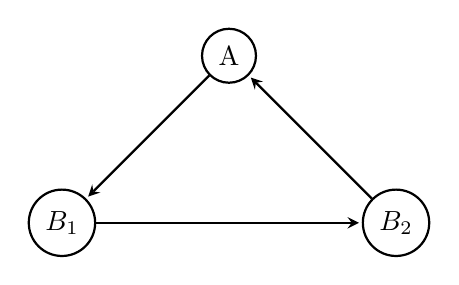
\begin{tikzpicture}[->, >=stealth, shorten >=1pt,auto,node distance=3cm,
                thick,main node/.style={circle,draw,}]

                \node[main node] (1) {A};
                \node[main node] (2) [below left of=1] {$B_1$};
                \node[main node] (3) [below right of=1] {$B_2$};

                \path[every node/.style={font=\sffamily\small}]
                (1) edge node [left] {} (2)
                (2) edge node [right] {} (3)
                (3) edge node [right] {} (1);
            \end{tikzpicture}
        \end{center}

        This would suggest that $A$, $B_1$, and $B_2$ are the same size. However, left multiplication by $a$ gives us 
        \[A \longrightarrow B_1 \cup B_2 \cup \overline A\]
        where $\overline A$ is some small extra subset of $A$.

        But this means that we can continuous apply $a$ and $b$ to get multiple copies of $A$. However, this idea is completely unmoored from space. Let's try to put this geometrically. 

        Consider a group action of $G$ on the unit ball $\beta$. Let $a$ act by a rotation of order $2$ (i.e. 180 degree rotation) and $b$ act by a rotation of order $3$ (i.e. 120 degree rotation) on two arbitrary fixed axes. 

        Now cut out the axis of rotation of every element of $G$. Now we partition this depleted ball into its orbits and use the Axiom of Choice to pick one element from each (countable) orbit.

        Each of those points is collected into a ``magic set'' $M$ which is a union of points, 1 from each orbit. Since each orbit is countably large, it is functionally a copy of the group so 
        \begin{gather*}
            A = A(M)\\
            B_1 = B_1(M)\\
            B_2 = B_2(M)
        \end{gather*}

        So the depleted ball now looks like 
        \begin{center}
            \usetikzlibrary{calc}
            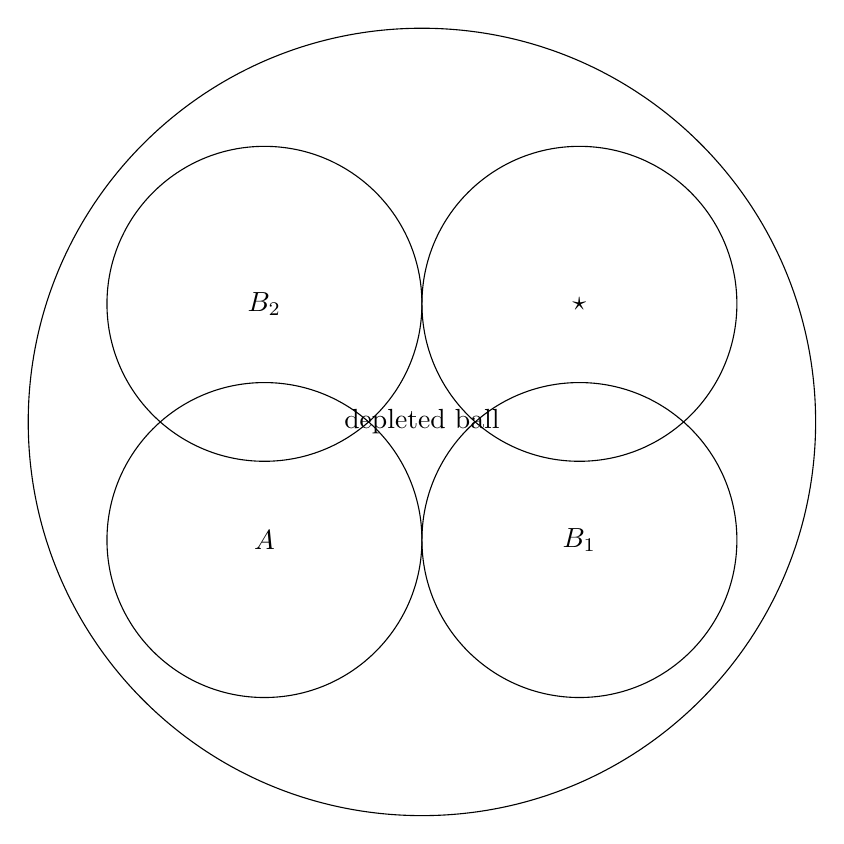
\begin{tikzpicture}
                % Draw the outer circle
                \draw (0,0) circle (5cm) node{depleted ball};
            
                \draw (-2, -1.5) circle (2cm) node{$A$};
                \draw (2, -1.5) circle (2cm) node{$B_1$};
                \draw (-2, 1.5) circle (2cm) node{$B_2$};
                \draw (2, 1.5) circle (2cm) node{$\star$};
            \end{tikzpicture}
        \end{center}

        Thus, using just isometries, we can create one depleted ball into two depleted balls plus some other stuff:
        \begin{align*}
            \beta' &= A\sqcup B_1 \sqcup B_2\\
                &= A \sqcup A \sqcup A\\
                &= B_1 \sqcup B_2 \sqcup B_1 \sqcup B_2 \sqcup  B_1 \sqcup B_2 \sqcup \star\\
                &= A \sqcup B_1 \sqcup B_2 \sqcup A \sqcup B_1 \sqcup B_2 \sqcup \star \\
                &= \beta' \sqcup \beta' \sqcup \star
        \end{align*}

        But we can also turn a solid ball into a depleted ball and then into many depleted balls!

\chapter*{Rings - Part II}
\section*{Lecture 21: Nov 28}
    \subsection*{Motivation}
        In $\Z$, things can be uniquely factored into primes (up to $\pm 1$ and order)

        In $\Z[\sqrt 5] = a + b\sqrt 5$, we have $6 = 2 \cdot 3 = (1 + \sqrt{-5})(1 - \sqrt{-5})$ and these are all irreducible. So numbers can be factored but not uniquely. 
        
        In $R = \{a_1 t^{e_1} + \dots + a_n t^{e_n}: \; a_i \in \R, \; e_i > 0, n \in \N \cup \{0\}\}$ (the ring of polynomials with real exponents). Notice that $t$ is not a unit in this ring (because $t\cdot t^{-1} = 1$ but $t^{-1} \not \in R$). We can factor $t = t^{1/4} \cdot t^{1/4}$ but this can further be factored infinitely.

    \subsection*{Definitions}
        \textbf{Ideal:} an \emph{ideal} is an abelian subgroup of a ring under addition with the absorber property. 

        \textbf{Principal Ideals:} $aR = \{ar \; | \; r \in R\}$

        \textbf{PID:} $R$ is a PID (principal ideal domain) if all ideals are principal. (We also assume it is an integral domain ($ab = 0 \implies a = 0 \text{ or } b = 0$))

        In any integral domain $R$, there are three kinds of elements:
        \begin{itemize}
            \item \emph{Units}: $u \in R: uv = 1$ for some $v \in R$ 
            \item \emph{Non-units}
            \item $0$
        \end{itemize}

        \textbf{Reducible:} a non-unit $p$ is \emph{reducible} if $p = ab$, where $a$, $b$ are non-units.

        \textbf{Irreducible:} $p$ is \emph{irreducible} if $p$ is not reducible
    
        \textbf{Associates:} $a$ and $b$ are \emph{associates} if $a = ub$ for some unit $u$ 

        \emph{Remark:} being associates is an equivalence relation because 
        \begin{align*}
            a &= 1a\\
            a &= ub \implies u^{-1}a = b\\
            a &= ub, \; b = vc \implies a = uvc
        \end{align*}

        \textbf{UFD:} $R$ is a UFD (unique factorization domain) if 
        \begin{enumerate}
            \item every non-unit factors into finitely many irreducibles 
            \item the factoring is unique up to units and reordering
        \end{enumerate}

    \subsection*{Theorem}
        \begin{tbox}{gray}{\textbf{Theorem}: If a ring is a PID, it is a UFD}
            \emph{Proof:} Call $a \in R$ ``bad'' if $a$ is a non-unit that does not factor into irreducibles. 

            Assume $a$ factors. We will denote the bad elements in red. 
            \begin{center}
                \begin{tikzpicture}[
                    level distance=1.5cm,
                    level 1/.style={sibling distance=3cm},
                    level 2/.style={sibling distance=1.5cm}]
                    \node[text=red] {$a$}
                    child {node {$a_1$}}
                    child {node[text=red] {$a_2$}
                        child {node {$a_{21}$}}
                        child {node[text=red] {$a_{22}$}
                            child {node {$a_{221}$}}
                            child {node[text=red] {$a_{222}$}}
                        }
                    };
                \end{tikzpicture}
            \end{center}

            Which gives an infinite tree of bad elements such that $a_2 \mid a$, $a_{22} \mid a_2$, $a_{222} \mid a_{22}$, etc. 

            Consider the ideals $I_0 = aR, I_1= a_2R, I_2 = a_{22}R, I_3 = a_{222}R, \dots$.
            
            Clearly, 
            \[I_0 \subset I_1 \subset I_2 \subset I_3\]

            \tcbbreak
            \begin{tcolorbox}[colback=gray!5!white,colframe=gray!75!black,
                title= \emph{Lemma:} $I_k \neq I_{k + 1}$]
                
                \emph{Proof:} Refer back to the tree diagram. Suppose $I_1 \subset I_0$ so $a_2 \in aR$. But then 
                \[a_2 = ac = a_1 a_2c = a_2 a_1 c\] 
                (by commutativity). We can do cancellation via 
                \[a_2a_1c = a_2(a_1(-1)) = 0 \implies a_2\ neq 0 \implies a_1(-1) = 0 \implies a_1c = 1\]
                Then $a_1c = 1 \implies a_1$ is a unit. But this is a contradiction of $a$'s badness. 
            \end{tcolorbox}

            Then, 
            \[J = \bigcup I_k\] 
            is also an ideal. 
            
            Then because $R$ is a PID, 
            \[J = cR \quad c \in J \implies c \in I_k\]
            for some $I_k$. 
            
            Since $I_k$ is an ideal, 
            \[rc \in I_k \; \forall r \in R \implies J = I_k\]

            But since $J$ is the union of all the $I_k$, $I_{k+1} \subset I_k$ but we also have $I_k \subset I_{k+1}$ so $I_k = I_{k+1}$ which is a contradiction.

            
            \begin{tcolorbox}[colback=gray!5!white,colframe=gray!75!black,
                title={\emph{Lemma:} In a PID, if $p$ irreducible and $p \mid ab$, then $p \mid a$ or $p \mid b$}]

                \emph{Proof:} Look at the ideal $\{mp + na \; | \; m, n \in R\} = I$. $I = cR$ since $R$ is a PID. 

                \textbf{Case 1:} $c$ is not a unit. 
                
                Then $p = rc$ for some $r$. Since $p$ is irreducible, $r$ is a unit so 
                \[a = sc = (sr^{-1})p \implies p \mid a\]

                \textbf{Case 2:} $c$ is a unit. 

                Then 
                \[Rc = R \implies 1 \in I\] 
                so $ma + np = 1$ for some $m, n \in $. We can multiply by $B$ so 
                \[mab + nbp = b\]
                $p$ divides both terms on the left so $p \mid b$. $\qed$
            \end{tcolorbox}

            \textbf{Back to the proof:} We assume that 
            \[a_1 \dots a_n = b_1 \dots b_m\]
            so 
            \[a_1 \mid b_1 \dots b_m\]
            After reordering, 
            \[a_1 \mid b_1 \implies b_1 = ua_1 \implies a_1 \text{ and } b_1 \text{ are associates}\]

            Using $b_1 = ua_1$, 
            \begin{align*}
                a_1 a_2 \dots a_n &= a_1(b_2u) b_3 \dots b_m\\
                a_2 \dots a_n &= (b_2u)b_3 \dots b_m\\
                &\vdots
            \end{align*}
            so we can repeat this process until we get $m = n$ and after reordering, $a_i$ and $b_i$ are associates. $\qed$
    \end{tbox}
       
\section*{Lecture 22: Nov 30} 
    \subsection*{Review}
        \textbf{Principal Ideal Domain:} a ring which is an integral domain and all ideals are principal.

        \textbf{Theorem:} If $R$ is a principal ideal domain, it is a unique factorization domain 
        
        \textbf{Remark:} UFD $\not \implies$ PID

    \subsection*{Euclidean Domains}
        \textbf{Example 1:} the integers $\Z$ is a Euclidean domain with $\sigma(n) = \abs n$. 
    
        This function has the properties that $\sigma(mn) \geq \sigma(m)$ and that given $a, b$ we can write $a = kb + r$ where $r = 0$ or $\sigma(r) < \sigma(b)$

        \textbf{Example 2:} $\Q[x]$ has $\sigma(a_n x^n + \dots + a_0) = n$ if $a_n \neq 0$ so $\sigma(p) = \deg(p)$ 

        Again, we have $\sigma(mn) \geq \sigma(m)$ and division works via the polynomial division algorithm 

        \textbf{Example 3:} $\Z[i] = \{a + bi \; | \; a, b \in \Z\}$ is a Euclidean domain with $\sigma(a + bi) = a^2 + b^2$.

        \textbf{Example 4:} $\Z[-\sqrt 5]$ is \textbf{not} a Euclidean domain 
        
        \textbf{Definition:} a Euclidean Domain is an integral domain with a size function $\sigma: R \diagdown \{0\} \to \{0, 1, 2, \dots\}$ such that
        \begin{enumerate}
            \item 
            \[\sigma(mn) \geq \sigma(m) \quad \forall m,n \in \R \diagdown \{0\}\]
            \item Given $a, b \in R - \{0\}$ we can write 
            \[a = kb + r \quad \begin{cases}
                r = 0 \text{ OR}\\
                \sigma(r) < \sigma(b)
            \end{cases}\]
        \end{enumerate}

        \begin{tbox}{gray}{\textbf{Theorem:} If a ring is a Euclidean Domain, it is a PID}
            \emph{Proof:} Let $I \neq \{0\}$ be an ideal. Since $\sigma$ is in the integers, there is a notion of a ``smallest element.'' Let $b \in I$ be an element which minimized $\sigma$ on $I$. 

            Let $a \in I$ be any other element. We have 
            \[a = kb + r\]
            where $r = 0$ or $\sigma(r) < \sigma(b)$. But $r = a - kb \in I$ so $r \in I$. But $\sigma(r) < \sigma(b)$ contradicts minimality of $b$. So $r = 0$ and $a = kb$. $\qed$
        \end{tbox}

    \subsection*{Unique Factorization in $\Z[i]$}
        \begin{align*}
            &3 \text{ irreducible}\\
            &5 = (1 + 2i)(1 - 2i) = (2 + i)(2 - i) \quad \text{(same up to associates)}\\
            &7 \text{ irreducible}\\
            &11 \text{ irreducible}\\
            &13 = (2 + 3i)(2 - 3i)\\
            &17 = (4 + i)(4 - i)
        \end{align*}

        But notice! 
        \begin{center}
            \begin{tabular}{|c|c|}
                \hline 
                $n$ & $n \mod 4$\\
                \hline
                3 & 3\\
                5 & 1\\ 
                7 & 3\\
                11 & 3\\
                13 & 1\\
                17 & 1\\
                \hline
            \end{tabular}
        \end{center}
        Which seems to suggest that $p$ is reducible in $\Z[i]$ if and only if $p \equiv 1 \mod 4$.

        \begin{tbox}{gray}{\textbf{Theorem:} if $p \in \Z$ is prime and $p \equiv 1 \mod 4$, then $p = a^2 + b^2$}
            \emph{Proof:} If $p$ is irreducible, then 
            \[\Z[i]/p\Z[i]\]
            would be a field and thus have no zero divisors.    
            
            Consider $p = 5$. Then $2^2 \equiv -1 \mod 5$ and 
            \[2^2 + 1 \equiv 0 \mod 5 \implies (2 + i)(2 - i) = 0\]
            and this is precisely a zero divisor so $p$ is not irreducible. 

            Generally, take $(\Z/p)^* = \{1, 2, \dots,\; \frac{p-1}{2}, - \frac{p-1}{2}, \dots, \; -1\}$. Because $p \equiv 1 \mod 4$, there is an odd number of elements in this set. If we take out $1$ and $-1$, the positive even half is the same size as the negative even half so the product of all elements except $\pm 1$ is $-1$ (mod p). 

            Eventually, we get $\alpha (-\alpha) \equiv 1 \mod 13 \implies \alpha^2 + 1 \equiv 0 \mod 13 \implies (\alpha + 1)(\alpha - 1) = 0 \qed$ 
        \end{tbox}

\section*{Lecture 23: Dec 05}
    \subsection*{The Two Square Theorem}
        \begin{tbox}{gray}{\textbf{Theorem:} if $p$ is a prime with $p \equiv 1\mod 4$, then $p = a^2 + b^2$ for some $a, b \in \Z$}
            \emph{Proof:}

            \begin{tbox}{gray}{\emph{Lemma:} $\alpha^2 + 1 \equiv 0$ for some $\alpha \in \Z/p$}
                \emph{Proof:}
                \begin{enumerate}
                    \item the product of all elements in $(\Z/p)^* = -1$ 
                    \item \[(1 \cdot 2 \dots \frac{p-1}{2})(-1 \cdot -2 \dots -\frac{p-1}{2}) = -1\]
                    \item \[\underbrace{(2 \dots \frac{p-1}{2})}_{\alpha}\underbrace{(-2 \dots -\frac{p-1}{2})}_{\alpha}  =1\]
                \end{enumerate}

                So $(\alpha)(-\alpha) = 1 \implies \alpha^2 = -1$ in $\Z/p$. $\qed$
            \end{tbox}
        
            Let $R = \Z[i]$. $R$ is a Euclidean domain so it is a PID. 
            
            Consider $R/pR$. It has zero divisors:
            \[(\alpha + i)(\alpha - i) = \alpha^2 + 1 \equiv 0 \mod p\]

            Thus, $R/pR$ is not a field, so $pR$ is not maximal. Thus, there is some ideal $I$ such that 
            \[pR \subsetneq I \subsetneq R\]
            so 
            \[pR \subseteq cR \subseteq R \]

            Since it is a subset, $p \in cR$ so $p = cd$ for some $d \in R$. But then 
            \[p^2 = \sigma(p) = \sigma(cd) = \sigma(c) \sigma(d)\]
            where $\sigma(\alpha) = \abs{\alpha}^2$

            So we have two cases:
            \begin{enumerate}
                \item $\sigma(c) = 1 \implies c$ is a unit so $cR = R$ (Contradiction)
                \item $\sigma(c) = p^2 \implies \sigma(d) = 1 \implies d$ is a unit so $cR = pR$ (Contradiction)
            \end{enumerate}

            Therefore, $\sigma(c) = p$. By definition of $\sigma$, $c = a + bi$ so $p = a^2 + b^2$. $\qed$
        \end{tbox}

    \subsection*{The Four Square Theorem}
        \begin{tbox}{gray}{\textbf{Theorem:} Every positive integer is the sum of four squares}
            \textbf{Proof:} Let $N(q) = N(a + bi + cj + dk) = a^2 + b^2 + c^2 + d^2 = q\overline{q}$. 

            Generally for quaternions, we have that $\overline{qr} = (\bar r)(\bar q)$ so 
            \[N(qr)  = qr\, \overline{qr} = qr \, \bar r\, \bar q = q N(r)\, \bar q = q\, \bar q N(r) = N(q)N(r)\] 

            Since the theorem is equivalent to saying that every integer is the norm of an integer quaternion, this factoring property means that it is sufficient to prove the theorem for odd primes (as everything else can just be multiplied up and we know that $2 = 1^2 + 1^2 + 
            0^2 + 0^2$)

            \begin{tbox}{gray}{\emph{Lemma:} for $p$ an odd prime $\exists \alpha, \beta: 1 + \alpha^2 + \beta^2 \equiv 0 \mod p$. }
                \emph{Proof:} Consider $A = \{\alpha^2 \mod p\}$ and $B = \{-1 - \beta^2 \mod p\}$. Both sets have $\frac{p+1}{2}$ elements (which is more than $p/2$) so they must intersect. Thus, there exists $\alpha, \beta$ for which $\alpha^2 = -1 \beta^2 \mod p$. Rearranging gives $1 + \alpha^2 + \beta^2 \equiv 0 \mod p. \qed$
            \end{tbox}

            We now introduce the \textbf{Hureuicz quaternions} where 
            \[\begin{cases}
                a, b, c, d \in \Z\\ 
                a, b, c, d \text{ are odd half-integers}
            \end{cases}\]
            whose units are the expected $\pm 1, \pm i, \pm j, \pm k$ but also $\frac{1}{2} + \frac{1}{2}i + \frac{1}{2}j + \frac{1}{2}k$ and all possible permutations of signs of that one (notice the norm is $1$). 

            It is relatively easy to prove that these are a ring but it is not a commutative ring, so it is not a Euclidean domain. However, it is a \emph{Left Euclidean Domain}. Though we will not prove it, this does imply that it is also a left principal idea. 

            Consider now $R/Rp$. It has zero divisors -- $(1 + ai + bj)(1 - ai - bi) \equiv 0 \mod p$ -- so it is not a \emph{division ring} (non-commutative field) and thus $Rp$ is not a maximal ideal: 
            \[Rp \subsetneq I \subsetneq R\] 
            $I$ is an ideal so it is also a left ideal so $I = Rc$ for some $c \in R$.

            Similar argument to the two square theorem shows that $p = N(\alpha)$ for $\alpha \in R$.

            Thus, we have successfully showed that every integer is the norm of a Hureuicz quaternion. All that remains is to show that it works for integer quaternions. 

            Notice 
            \[p = N(a) = N(a \omega)\]
            for any unit $\omega$. We pick $\omega$ so $\omega + \alpha$ is all even integers. 

            For example, if $\alpha = \frac{3}{2} - \frac{7}{2}i + \frac{5}{2}j + \frac{13}{2}k$, we can choose $\omega = \frac{1}{2} - \frac{1}{2}i - \frac{1}{2}j - \frac{1}{2}k$ so 
            \[\alpha + \omega = 4 - 4i + 2i + 6i\]
            
            Then we can use an orthonormal matrix on one of the quaternions
            \[\frac{1}{2}\begin{pmatrix}
                1 & 1 & 1 & 1\\
                1 & 1 & -1 & -1\\
                1 & -1 & 1 & -1\\
                1 & -1 & -1 & 1
            \end{pmatrix} \begin{pmatrix}
                a/2 \\ 
                b/2\\ 
                c/2\\ 
                d/2
            \end{pmatrix} = \begin{pmatrix}
                \frac{1}{4}(a + b + c + d) = \alpha\\ 
                \frac{1}{4}(a + b - c - d) = \beta\\
                \frac{1}{4}(a - b + c - d) = \gamma\\
                \frac{1}{4}(a - b - c + d) = \delta
            \end{pmatrix}\]
            So all the entries are divisible by $4$. Thus, 
            \[p = N(\alpha + \beta i + \gamma j + \delta k)\] 
            and we have any prime as the norm of an integer quaternion. $\qed$
        \end{tbox}

\chapter*{Fields - Part II}
\section*{Lecture 24: Dec 07}
    \begin{tbox}{gray}{\textbf{Theorem:} If $p$ is prime and $n \geq 1$, there exists a field of order $p^n$}
        \emph{Proof 1 (Calculus):} We generalize the derivative to $F[x]$:
        \[\frac{d}{dx}(a_0 + a_1 x + \dots + a_n x^n) := a_1 + 2a_2 x + 3a_3x^2 + \dots + na_nx^{n-1}\]
        \[\frac{d}{dx}(f +g) := \frac{df}{dx} + \frac{dg}{dx}\]
        \[\frac{d}{dx}(fg) := f\frac{dg}{dx} + g \frac{df}{dx}\]

        Now suppose we have $p(x) \in F[x]$ and it factors completely so we can write 
        \[p(x) = (x - a_1) \dots (x - a_n) = (x - a_1)q_0(x)\]
        If $a_1$ is a multiple root, we can use the product rule and take 
        \[\frac{dp}{dx} = (x - a_1)^2 q_1(x) + 2(x- a_1) q_2(x) = (x - a_1) q_3(x)\]
        (where each of the $q$s are just the product of the rest of the terms)

        Thus, if $p$ has a multiple root, then $p$ and $\frac{dp}{dx}$ have a common factor. Thud, $p$ is not a unit. 

        \emph{Example:} $p(x) = x^p - x, \quad \frac{dp}{dx} = px^{p-1} - 1 = -1 \implies p$ has $p$ distinct roots in $F$.

        Now we take the polynomial $p(x) = x^{p^n} - x \in \Z/p[x]$. There exists a field $K$ that has all roots of $p$. We also know $\frac{dp}{dx} = p^nx^{p^n-1} -1 = -1$ so $p$ has $p^n$ distinct roots. 

        Let $F \subset K$ be the union of all roots. We know:
        \begin{enumerate}
            \item $\abs{F} = p^n$
            \item $0 \in F$ and $1 \in F$
            \item $a, b \in F \implies ab \in F$ because $(ab)^{p^n} = a^{p^n}b^{p^n} = (-a)(-b) = ab$
            \item $a \in F \implies -a \in F$ because $(-a)^{p^n} = -a^{p^n} = -(-a) = a$
            \item $a \in F \implies a^{-1} \in F$ because $(a^{-1})^{p^n} \cdot a^{p^n} = a^{-1} \cdot a = 1$
            \item $(a + b)^p = a^p + \binom{p}{1} a^{p-1}b + \binom{p}{2}a^{p-2}b^2 + \dots + \binom{p}{p-1}ab^{p-1} + b^p = a^p + b^p$ because $p \mid \binom{p}{k}$ for $1 \leq k \leq p-1$. So $a, b \in F \implies (a + b)^{p^n} = a^{p^n} + b^{p^n} = a + b \in F$.
        \end{enumerate}
        Thus, $F$ is a field of order $p^n$. $\qed$ 
    \end{tbox}

\end{document}  


 